\documentclass[a4paper, 11pt]{article}
\input{macro/package.tex}
\input{macro/environement}
% Header et footer

\pagestyle{fancy}
\fancyhead{}
\fancyfoot{}
\renewcommand{\headwidth}{\textwidth}
\renewcommand{\footrulewidth}{0.4pt}
\renewcommand{\headrulewidth}{0pt}
\renewcommand{\footruleskip}{5px}

\fancyfoot[R]{Olivier Glorieux}
%\fancyfoot[R]{Jules Glorieux}

\fancyfoot[C]{ Page \thepage }
\fancyfoot[L]{1BIOA - Lycée Chaptal}
%\fancyfoot[L]{MP*-Lycée Chaptal}
%\fancyfoot[L]{Famille Lapin}

\input{macro/newcommand.tex}
\geometry{hmargin=2.0cm, vmargin=2.0cm}
\newcommand{\type}{TD }
\excludecomment{correction}
%\renewcommand{\type}{Correction TD }


\begin{document}

\title{\type  2 - Trigonométrie}


%----------------------------------------------------------------------------------------------
%-----------------------------------------------------------------------------------------------
\section*{Entraînements}



\begin{exercice}  \;
Calculer les r\'eels suivants: $\cos{\left(\ddp\frac{\pi}{12}\right)},\ \sin{\left(\ddp\frac{\pi}{12}\right)},\ \cos{\left(\ddp\frac{7\pi}{12}\right)},\ \cos{\left(\ddp\frac{\pi}{8}\right)}\ \hbox{et}\ \sin{\left(\ddp\frac{\pi}{8}\right)} .$
\end{exercice}
\begin{correction}  \;
\begin{itemize}
\item[$\bullet$] \textbf{Calcul de $\mathbf{\cos{\left(\ddp\frac{\pi}{12}\right)}}$:} on a $\ddp \frac{pi}{3}-\frac{\pi}{4} = \frac{\pi}{12}$, donc :
$$\ddp \cos\left(\ddp\frac{\pi}{12}\right) = \cos\left(\frac{\pi}{3}-\frac{\pi}{4}\right) = \cos \left(\frac{\pi}{3}\right)\cos \left(\frac{\pi}{4}\right) + \sin \left(\frac{\pi}{3}\right)\sin \left(\frac{\pi}{4}\right),$$
soit apr\`es simplification : \fbox{$\ddp \cos \left(\frac{\pi}{12}\right) = \frac{\sqrt{2}(1+\sqrt{3})}{4}$}.
\item[$\bullet$] \textbf{Calcul de $\mathbf{\sin{\left(\ddp\frac{\pi}{12}\right)}}$:}  de m\^eme, on a 
$$\ddp \sin\left(\ddp\frac{\pi}{12}\right) = \sin\left(\frac{\pi}{3}-\frac{\pi}{4}\right) = \sin \left(\frac{\pi}{3}\right)\cos \left(\frac{\pi}{4}\right) - \cos \left(\frac{\pi}{3}\right)\sin \left(\frac{\pi}{4}\right),$$
soit apr\`es simplification : \fbox{$\ddp \sin \left(\frac{\pi}{12}\right) = \frac{\sqrt{2}(\sqrt{3}-1)}{4}$}.
\item[$\bullet$] \textbf{Calcul de $\mathbf{\cos{\left(\ddp\frac{7\pi}{12}\right)}}$:} \`a partir du calcul pr\'ec\'edent, on a :
$$\ddp \cos{\left(\ddp\frac{7\pi}{12}\right)} = \cos{\left(\ddp\frac{\pi}{12}+\frac{\pi}{2}\right)} = -\sin{\left(\ddp\frac{\pi}{12}\right)} = \fbox{$\ddp \frac{\sqrt{2}(1-\sqrt{3}}{4}$}$$
%-----
\item[$\bullet$] \textbf{Calcul de $\mathbf{\cos{\left(\ddp\frac{\pi}{8}\right)}}$ et $\mathbf{\sin{\left(\ddp\frac{\pi}{8}\right)}}$:}  Il suffit de remarquer que: $\ddp\frac{\pi}{8}=\frac{\pi}{4}\times \demi$. On pose alors $\theta=\ddp\frac{\pi}{8}$ et on obtient par la formule de duplication des angles : $\cos{(2\theta)}=2\cos^2{(\theta)}-1.$
Ainsi, 
$$\cos^2{\left(\ddp\frac{\pi}{8}\right)}=\ddp\frac{\cos{\left(\frac{\pi}{4}\right)}+1}{2}=\ddp\frac{\sqrt{2}+2}{4}.$$
Le r\'eel $\ddp\frac{\pi}{8}$ est dans l'intervalle $\left\lbrack 0,\ddp\frac{\pi}{2}\right\rbrack$ et le cosinus est positif sur cet intervalle, ainsi: 
\begin{equation*}
\fbox{
$\cos{\left(\ddp\frac{\pi}{8}\right)}=\ddp\sqrt{\frac{\sqrt{2}+2}{4}}.$
}
\end{equation*}
Une fois le cosinus connu, le sinus se d\'eduit par la formule $\cos^2{(x)}+\sin^2{(x)}=1$. On obtient ainsi, 
$$\sin^2{\left(\ddp\frac{\pi}{8}\right)}=1-\ddp \frac{\sqrt{2}+2}{4} = \frac{2-\sqrt{2}}{4}.$$
L\`a encore, le sinus \'etant positif sur l'intervalle $\left\lbrack 0,\ddp\frac{\pi}{2}\right\rbrack$, on obtient: 
\begin{equation*}
\fbox{
$\sin{\left(\ddp\frac{\pi}{8}\right)}=\ddp\sqrt{\frac{2-\sqrt{2}}{4}}.$
}
\end{equation*}
\end{itemize}
\end{correction}






%------------------------------------------------------------------------------------------
\begin{exercice}  \;
R\'esoudre sur $\R$ les \'equations suivantes et repr\'esenter les solutions sur le cercle trigonom\'etrique:
\begin{enumerate}
\begin{minipage}[t]{0.45\textwidth}
\item $\cos{(5x)}=\ddp\frac{\sqrt{3}}{2}$
\item $\sin{(4x)}=-\ddp\frac{1}{2}$
\end{minipage}
\begin{minipage}[t]{0.45\textwidth}
\item $\tan{\left(\ddp\frac{x}{2}\right)}=-1$
\item $\tan{(2x)}=-\sqrt{3}$
\end{minipage}
\end{enumerate}
\end{exercice}
\begin{correction}  \;
Il s'agit dans cet exercice d'\'egalit\'es trigonom\'etriques fondamentales que l'on r\'esout donc en appliquant la m\'ethode du cours. 
\begin{enumerate}
 \item \textbf{R\'esolution de $\mathbf{\cos{(5x)}=\ddp\frac{\sqrt{3}}{2}}$:}
L'\'egalit\'e est de type \'equation fondamentale.
$$\begin{array}{lll}
\cos{(5x)}=\ddp\frac{\sqrt{3}}{2}&\Leftrightarrow &\cos{(5x)}= \cos{\left(\ddp\frac{\pi}{6}\right)}
\Leftrightarrow  \left\lbrace\begin{array}{l}
\exists k\in\Z,\ 5x=\ddp\frac{\pi}{6}+2k\pi\vsec\\
\hbox{ou}\vsec\\
\exists k\in\Z,\ 5x=-\ddp\frac{\pi}{6}+2k\pi.
\end{array}\right.
\end{array}$$
\begin{minipage}[c]{0.45\linewidth}
On obtient donc
\begin{equation*}
\fbox{
$\mathcal{S}=\left\lbrace \ddp\frac{\pi}{30}+\frac{2k\pi}{5},\ k\in\Z\right\rbrace\cup\left\lbrace -\ddp\frac{\pi}{30}+\frac{2k\pi}{5},\ k\in\Z\right\rbrace.$
}
\end{equation*}
\end{minipage}
\quad

\begin{center}
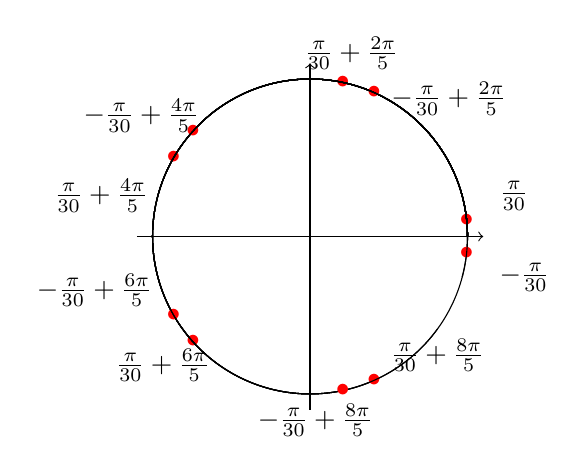
\begin{tikzpicture}[scale=2]
%Axes
\draw [->] (-1.1,0) -- (1.1,0);
\draw [->] (0,-1.1) -- (0,1.1);
%Cercle
\draw (0,0) circle (1);
%Points
\draw (1,0) arc (0:6:1) node [red] {$\bullet$};
\draw (1,0) arc (0:15:1) node[right] {$\quad \ddp \frac{\pi}{30}$} ;
\draw (1,0) arc (0:78:1) node [red] {$\bullet$};
\draw (1,0) arc (0:85:1) node[above] {$\quad\quad \ddp \frac{\pi}{30}+\frac{2\pi}{5}$} ;
\draw (1,0) arc (0:150:1) node [red] {$\bullet$};
\draw (1,0) arc (0:165:1) node[left] {$\ddp \frac{\pi}{30}+\frac{4\pi}{5}$} ;
\draw (1,0) arc (0:222:1) node [red] {$\bullet$};
\draw (1,0) arc (0:235:1) node[left] {$\ddp \frac{\pi}{30}+\frac{6\pi}{5}$} ;
\draw (1,0) arc (0:294:1) node [red] {$\bullet$};
\draw (1,0) arc (0:324:1) node[below] {$\ddp \frac{\pi}{30}+\frac{8\pi}{5}$} ;
\draw (1,0) arc (0:-6:1) node [red] {$\bullet$};
\draw (1,0) arc (0:-15:1) node[right] {$\quad \ddp - \frac{\pi}{30}$} ;
\draw (1,0) arc (0:66:1) node [red] {$\bullet$};
\draw (1,0) arc (0:45:1) node[above] {$\quad\quad \ddp -\frac{\pi}{30}+\frac{2\pi}{5}$} ;
\draw (1,0) arc (0:138:1) node [red] {$\bullet$};
\draw (1,0) arc (0:130:1) node[left] {$\ddp -\frac{\pi}{30}+\frac{4\pi}{5}$} ;
\draw (1,0) arc (0:210:1) node [red] {$\bullet$};
\draw (1,0) arc (0:200:1) node[left]  {$\ddp -\frac{\pi}{30}+\frac{6\pi}{5}$} ;
\draw (1,0) arc (0:282:1) node [red] {$\bullet$};
\draw (1,0) arc (0:272:1) node[below] {$\ddp -\frac{\pi}{30}+\frac{8\pi}{5}$} ;
\end{tikzpicture}
\end{center}

Pour savoir combien de points tracer sur le cercle pour chaque ensemble de solutions, on cherche la premi\`ere valeur de $k$ pour laquelle on retombe sur la solution de d\'epart modulo $2\pi$. Par exemple, pour le premier ensemble de solution, on cherche $k$ tel que $\ddp \frac{2k\pi}{5} = 2\pi$, soit $k=5$ : on doit donc tracer $5$ points sur le cercle trigonom\'etrique. M\^eme chose pour le deuxi\`eme ensemble de solutions.
%------------------------------
\item  \textbf{R\'esolution de $\mathbf{\sin{(4x)}=-\ddp\frac{1}{2}}$:}
L'\'egalit\'e est de type \'equation fondamentale.
$$\begin{array}{lll}
\sin{(4x)}=-\ddp\frac{1}{2}&\Leftrightarrow &\sin{(4x)}= \sin{\left(-\ddp\frac{\pi}{6}\right)}
\Leftrightarrow  \left\lbrace\begin{array}{l}
\exists k\in\Z,\ 4x=-\ddp\frac{\pi}{6}+2k\pi\vsec\\
\hbox{ou}\vsec\\
\exists k\in\Z,\ 4x=\pi+\ddp\frac{\pi}{6}+2k\pi.
\end{array}\right.
\end{array}$$
\begin{minipage}[c]{0.45\linewidth}
On obtient donc
\begin{equation*}
\fbox{
$\mathcal{S}=\left\lbrace -\ddp\frac{\pi}{24}+\frac{k\pi}{2},\ k\in\Z\right\rbrace\cup\left\lbrace \ddp\frac{7\pi}{24}+\frac{k\pi}{2},\ k\in\Z\right\rbrace.$
}
\end{equation*}
\end{minipage}
\quad

\begin{center}
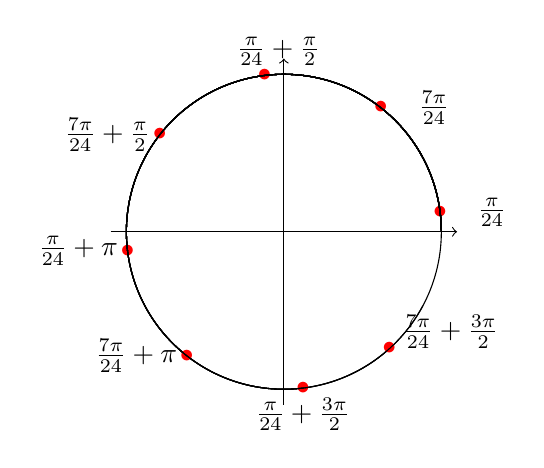
\begin{tikzpicture}[scale=2]
%Axes
\draw [->] (-1.1,0) -- (1.1,0);
\draw [->] (0,-1.1) -- (0,1.1);
%Cercle
\draw (0,0) circle (1);
%Points
\draw (1,0) arc (0:7:1) node [red] {$\bullet$};
\draw (1,0) arc (0:7:1) node[right] {$\quad \ddp \frac{\pi}{24}$} ;
\draw (1,0) arc (0:97:1) node [red] {$\bullet$};
\draw (1,0) arc (0:97:1) node[above] {$\quad \ddp \frac{\pi}{24}+\frac{\pi}{2}$} ;
\draw (1,0) arc (0:187:1) node [red] {$\bullet$};
\draw (1,0) arc (0:187:1) node[left] {$\ddp \frac{\pi}{24}+\pi$} ;
\draw (1,0) arc (0:277:1) node [red] {$\bullet$};
\draw (1,0) arc (0:277:1) node[below] {$\ddp \frac{\pi}{24}+\frac{3\pi}{2}$} ;
\draw (1,0) arc (0:52:1) node [red] {$\bullet$};
\draw (1,0) arc (0:52:1) node[right] {$\quad \ddp \frac{7\pi}{24}$} ;
\draw (1,0) arc (0:142:1) node [red] {$\bullet$};
\draw (1,0) arc (0:142:1) node[left] {$\quad \ddp \frac{7\pi}{24}+\frac{\pi}{2}$} ;
\draw (1,0) arc (0:232:1) node [red] {$\bullet$};
\draw (1,0) arc (0:232:1) node[left] {$\quad \ddp \frac{7\pi}{24}+\pi$} ;
\draw (1,0) arc (0:312:1) node [red] {$\bullet$};
\draw (1,0) arc (0:332:1) node[below]  {$\quad \quad \ddp \frac{7\pi}{24}+\frac{3\pi}{2}$} ;
\end{tikzpicture}
\end{center}

On remarque ici qu'il faut tracer $4$ points pour chaque ensemble de solutions : en effet, on doit chercher $k$ tel que $\ddp \frac{k \pi}{2} = 2 \pi$, soit $k=4$.
%-------------------------------------
\item \textbf{R\'esolution de $\mathbf{\tan{\left(\ddp\frac{x}{2}\right)}}$:}
L'\'egalit\'e est de type \'equation fondamentale. On peut commencer par chercher le domaine de d\'efinition de cette \'equation. On a, d'apr\`{e}s le domaine de d\'efinition de la tangente, que: $\ddp\frac{x}{2}\not= \ddp\frac{\pi}{2}+k\pi,\ k\in\Z\Leftrightarrow x\not= \pi+2k\pi,\ k\in\Z$. On r\'esout ensuite l'\'equation fondamentale et on v\'erifiera bien que les solutions trouv\'ees n'appartiennent pas \`{a} l'ensemble $\left\lbrace  \pi+2k\pi,\ k\in\Z \right\rbrace$. 
$$\begin{array}{lll}
\tan{\left(\ddp\frac{x}{2}\right)}=-1 &\Leftrightarrow & \tan{\left(\ddp\frac{x}{2}\right)}= \tan{\left(-\ddp\frac{\pi}{4}\right)}
\Leftrightarrow  \exists k\in\Z,\ \ddp\frac{x}{2}=-\ddp\frac{\pi}{4}+k\pi.\\
%&\Leftrightarrow & \begin{array}{|l|}
%\hline
%\exists k\in\Z,\ x=-\ddp\frac{\pi}{2}+2k\pi.\\
%\hline
%\end{array}
\end{array}$$
On obtient donc
\begin{equation*}
\fbox{
$\mathcal{S}=\left\lbrace -\ddp\frac{\pi}{2}+2k\pi,\ k\in\Z\right\rbrace.$
}
\end{equation*}
%-------------------------------------
\item \textbf{R\'esolution de $\mathbf{ \tan{(2x)}=-\sqrt{3}}$:}
L'\'egalit\'e est de type \'equation fondamentale.
On peut commencer par chercher le domaine de d\'efinition de cette \'equation. On a, d'apr\`{e}s le domaine de d\'efinition de la tangente, que: $2x\not= \ddp\frac{\pi}{2}+k\pi,\ k\in\Z\Leftrightarrow x\not= \ddp\frac{\pi}{4}+\ddp\frac{k\pi}{2} ,\ k\in\Z$. On r\'esout ensuite l'\'equation fondamentale et on v\'erifiera bien que les solutions trouv\'ees n'appartiennent pas \`{a} l'ensemble $\left\lbrace \ddp\frac{\pi}{4}+\ddp\frac{k\pi}{2},\ k\in\Z \right\rbrace$. 
$$\begin{array}{lll}
\tan{(2x)}=-\sqrt{3} &\Leftrightarrow & \tan{(2x)}= \tan{\left(-\ddp\frac{\pi}{3}\right)}
\Leftrightarrow  \exists k\in\Z,\ 2x=-\ddp\frac{\pi}{3}+k\pi.
\end{array}$$
\begin{minipage}[c]{0.45\linewidth}
On obtient donc
\begin{equation*}
\fbox{
$\mathcal{S}=\left\lbrace -\ddp\frac{\pi}{6}+\ddp\frac{k\pi}{2},\ k\in\Z\right\rbrace.$
}
\end{equation*}
\end{minipage}
\quad
\begin{minipage}[c]{0.45\linewidth}
\begin{center}
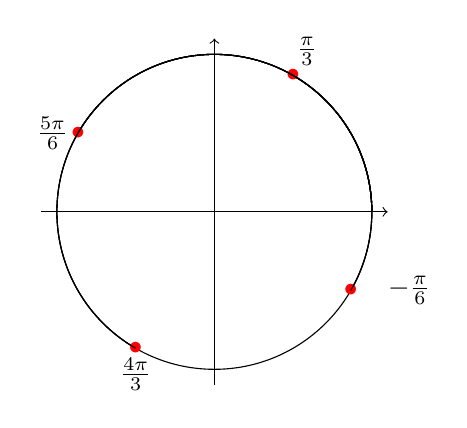
\begin{tikzpicture}[scale=2]
%Axes
\draw [->] (-1.1,0) -- (1.1,0);
\draw [->] (0,-1.1) -- (0,1.1);
%Cercle
\draw (0,0) circle (1);
%Points
\draw (1,0) arc (0:-30:1) node [red] {$\bullet$};
\draw (1,0) arc (0:-30:1) node[right] {$\quad \ddp -\frac{\pi}{6}$} ;
\draw (1,0) arc (0:60:1) node [red] {$\bullet$};
\draw (1,0) arc (0:60:1) node[above] {$\quad \ddp \frac{\pi}{3}$} ;
\draw (1,0) arc (0:150:1) node [red] {$\bullet$};
\draw (1,0) arc (0:150:1) node[left] {$\ddp \frac{5\pi}{6}$} ;
\draw (1,0) arc (0:240:1) node [red] {$\bullet$};
\draw (1,0) arc (0:240:1) node[below] {$\ddp \frac{4\pi}{3}$} ;
\end{tikzpicture}
\end{center}
\end{minipage}
\end{enumerate}
\end{correction}


%------------------------------------------------------------------------------------------
\begin{exercice}  \;
R\'esoudre dans $\R$, puis dans $\lbrack 0,2\pi\lbrack$ et enfin dans $\rbrack -\pi,\pi\rbrack$ les \'equations suivantes:
\begin{enumerate}
\noindent \begin{minipage}[t]{0.45\textwidth}
\item $\sin{x}-\cos{x}=\ddp\frac{\sqrt{6}}{2}$
\item $-\sqrt{3}\sin{x}+\cos{x}=\sqrt{2}$
\end{minipage}
\begin{minipage}[t]{0.45\textwidth}
\item $\sin{x}+\ddp\frac{1}{\sqrt{3}}\cos{x}=0$
\item $\cos{(2x)}+\sqrt{3}\sin{(2x)}=\sqrt{2}$
\end{minipage}
\end{enumerate}
\end{exercice}
\begin{correction}  \;
\begin{enumerate}
%--------------------------------------------------
\item \textbf{R\'esolution de $\mathbf{\sin{x}-\cos{x}=\ddp\frac{\sqrt{6}}{2}}$:}
On reconna\^{i}t la forme $a\cos{(x)}+b\sin{(x)}$, on applique donc la m\'ethode associ\'ee. On obtient alors
$$\begin{array}{lll} \sin{x}-\cos{x}=\ddp\frac{\sqrt{6}}{2} &\Leftrightarrow &\sqrt{2}\left( -\ddp\frac{1}{\sqrt{2}}\cos{(x)}+\ddp\frac{1}{\sqrt{2}}\sin{(x)}  \right)=\ddp\frac{\sqrt{3}\sqrt{2}}{2}\Leftrightarrow \cos{\left( x-\ddp\frac{3\pi}{4} \right)}=\ddp\frac{\sqrt{3}}{2}\vsec\\
&\Leftrightarrow& \left\lbrace\begin{array}{lllll} \exists k\in\Z,& x-\ddp\frac{3\pi}{4} &=&  \ddp\frac{\pi}{6}+2k\pi \vsec\\ \exists k\in\Z,& x-\ddp\frac{3\pi}{4} &=&  -\ddp\frac{\pi}{6}+2k\pi\end{array}\right. \end{array}$$ 
\begin{minipage}[c]{0.45\linewidth}
On obtient ainsi:
\begin{itemize}
\item[$\bullet$] Sur $\R$ : 
$$\fbox{$\mathcal{S}_\R=\left\lbrace \ddp\frac{11\pi}{12}+2k\pi,\ k\in\Z  \right\rbrace\cup \left\lbrace \ddp\frac{7\pi}{12}+2k\pi,\ k\in\Z  \right\rbrace.$}$$
 \item[$\bullet$] Sur $\lbrack 0,2\pi\lbrack$ comme sur $\rbrack -\pi,\pi\rbrack$ : 
 $$\fbox{$\mathcal{S}_{[0,2\pi[}=\mathcal{S}_{]-\pi,\pi]}= \left\lbrace \ddp\frac{7\pi}{12},\ddp\frac{11\pi}{12} \right \rbrace.$}$$
\end{itemize}
\end{minipage}
\quad

\begin{center}
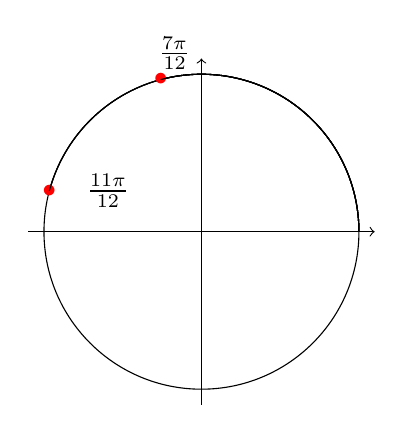
\begin{tikzpicture}[scale=2]
%Axes
\draw [->] (-1.1,0) -- (1.1,0);
\draw [->] (0,-1.1) -- (0,1.1);
%Cercle
\draw (0,0) circle (1);
%Points
\draw (1,0) arc (0:165:1) node [red] {$\bullet$};
\draw (1,0) arc (0:165:1) node[right] {$\quad \ddp \frac{11\pi}{12}$} ;
\draw (1,0) arc (0:105:1) node [red] {$\bullet$};
\draw (1,0) arc (0:105:1) node[above] {$\quad \ddp \frac{7\pi}{12}$} ;
\end{tikzpicture}
\end{center}

%--------------------------------------------------
\item  \textbf{R\'esolution de $\mathbf{ -\sqrt{3}\sin{x}+\cos{x}=\sqrt{2}}$:}
M\^{e}me m\'ethode que dans l'exemple pr\'ec\'edent. On obtient ainsi
\begin{itemize}
\item[$\bullet$] Sur $\R$ : 
$$\fbox{$\mathcal{S}_\R=\left\lbrace \ddp-\frac{7\pi}{12}+2k\pi,\ k\in\Z  \right\rbrace\cup \left\lbrace - \ddp\frac{\pi}{12}+2k\pi,\ k\in\Z  \right\rbrace .$}$$
\end{itemize}
\begin{minipage}[c]{0.45\linewidth}
\begin{itemize}
\item[$\bullet$] Sur $\lbrack 0,2\pi\lbrack$ : 
$$\fbox{$\mathcal{S}=\left\lbrace \ddp\frac{17\pi}{12},\ddp\frac{23\pi}{12} \right \rbrace.$}$$
\item[$\bullet$] Sur $\lbrack -\pi,\pi\lbrack$ :
$$\fbox{$\mathcal{S}=\left\lbrace -\ddp\frac{\pi}{12},-\ddp\frac{7\pi}{12} \right \rbrace.$}$$
\end{itemize}
\end{minipage}
\quad

\begin{center}
\begin{tikzpicture}[scale=2]
%Axes
\draw [->] (-1.1,0) -- (1.1,0);
\draw [->] (0,-1.1) -- (0,1.1);
%Cercle
\draw (0,0) circle (1);
%Points
\draw (1,0) arc (0:255:1) node [red] {$\bullet$};
\draw (1,0) arc (0:255:1) node[below] {$\quad \ddp - \frac{7\pi}{12}$} ;
\draw (1,0) arc (0:-15:1) node [red] {$\bullet$};
\draw (1,0) arc (0:-15:1) node[right] {$\quad \ddp - \frac{\pi}{12}$} ;
\end{tikzpicture}
\end{center}

%--------------------------------------------------
\item  \textbf{R\'esolution de $\mathbf{ \sin{x}+\ddp\frac{1}{\sqrt{3}}\cos{x}=0 }$:}
M\^{e}me m\'ethode que dans l'exemple pr\'ec\'edent. On a: 
$$\sin{x}+\ddp\frac{1}{\sqrt{3}}\cos{x}=0 \Leftrightarrow \cos{\left(  x-\ddp\frac{\pi}{3}\right)=0}\Leftrightarrow \exists k\in\Z,\ x-\ddp\frac{\pi}{3}=\ddp\frac{\pi}{2}+k\pi.$$ 
On obtient ainsi:\\
\begin{minipage}[c]{0.45\linewidth}
\begin{itemize}
\item[$\bullet$] Sur $\R$: \fbox{$\mathcal{S}=\left\lbrace \ddp\frac{5\pi}{6}+k\pi,\ k\in\Z  \right\rbrace.$}
\item[$\bullet$] Sur $\lbrack 0,2\pi\lbrack$: \fbox{$\mathcal{S}=\left\lbrace \ddp\frac{5\pi}{6},\ddp\frac{11\pi}{6} \right \rbrace.$}
\item[$\bullet$]  Sur $\lbrack -\pi,\pi\lbrack$: \fbox{$\mathcal{S}=\left\lbrace -\ddp\frac{\pi}{6},\ddp\frac{5\pi}{6} \right \rbrace.$}
\end{itemize}
\end{minipage}
\quad
-
\begin{center}
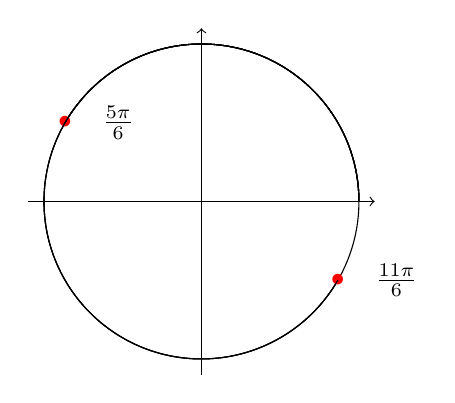
\begin{tikzpicture}[scale=2]
%Axes
\draw [->] (-1.1,0) -- (1.1,0);
\draw [->] (0,-1.1) -- (0,1.1);
%Cercle
\draw (0,0) circle (1);
%Points
\draw (1,0) arc (0:150:1) node [red] {$\bullet$};
\draw (1,0) arc (0:150:1) node[right] {$\quad \ddp \frac{5\pi}{6}$} ;
\draw (1,0) arc (0:330:1) node [red] {$\bullet$};
\draw (1,0) arc (0:330:1) node[right] {$\quad \ddp \frac{11\pi}{6}$} ;
\end{tikzpicture}
\end{center}

%---------------------------------------------------
\item \textbf{R\'esolution de $\mathbf{ \cos{(2x)}+\sqrt{3}\sin{(2x)}=\sqrt{2}  }$:}
Quitte \`{a} poser $X=2x$, l'\'egalit\'e est de type $a\cos{(X)}+b\sin{(X)}=c$, on applique donc la m\'ethode du cours. On se ram\`ene ainsi \`a l'\'equation fondamentale suivante:   $\cos{(X-\ddp\frac{\pi}{3})}=\ddp\frac{\sqrt{2}}{2}\Leftrightarrow \cos{(2x-\ddp\frac{\pi}{3})}=\ddp\frac{\sqrt{2}}{2}.$
Ainsi,
$$
\cos{(2x)}+\sqrt{3}\sin{(2x)}=\sqrt{2}\Leftrightarrow 
\left\lbrace
\begin{array}{l}
\exists k\in\Z,\ 2x-\ddp\frac{\pi}{3}=\ddp\frac{\pi}{4}+2k\pi\vsec\\
\hbox{ou}\vsec\\
\exists k\in\Z,\ 2x-\ddp\frac{\pi}{3}=-\ddp\frac{\pi}{4}+2k\pi.
\end{array}\right.
$$
On obtient ainsi:
\begin{itemize}
\item[$\bullet$] Sur $\R$ : \fbox{$\mathcal{S}=\left\lbrace x\in\R;\   \exists k\in\Z,\ x=\ddp\frac{7\pi}{24}+k\pi\right\rbrace\cup\left\lbrace x\in\R;\   \exists k\in\Z,\ x=\ddp\frac{\pi}{24}+k\pi\right\rbrace .$}
\end{itemize}
\begin{minipage}[c]{0.45\textwidth}
\begin{itemize}
\item[$\bullet$] Sur $\lbrack 0,2\pi\lbrack$ : \conclusion{$\mathcal{S}=\left\lbrace \ddp\frac{\pi}{24},\ddp\frac{7\pi}{24},\ddp\frac{25\pi}{24},\ddp\frac{31\pi}{24}   \right \rbrace.$}
\item[$\bullet$] Sur $]-\pi,\pi]$ : 

\conclusion{$\mathcal{S}=\left\lbrace -\ddp\frac{23\pi}{24},-\ddp\frac{17\pi}{24},\ddp\frac{\pi}{24},\ddp\frac{7\pi}{24}     \right\rbrace.$}
\end{itemize}
\end{minipage}


\begin{center}
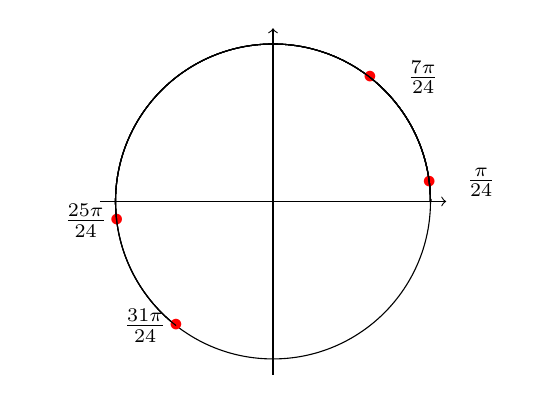
\begin{tikzpicture}[scale=2]
%Axes
\draw [->] (-1.1,0) -- (1.1,0);
\draw [->] (0,-1.1) -- (0,1.1);
%Cercle
\draw (0,0) circle (1);
%Points
\draw (1,0) arc (0:7:1) node [red] {$\bullet$};
\draw (1,0) arc (0:7:1) node[right] {$\quad \ddp \frac{\pi}{24}$} ;
\draw (1,0) arc (0:187:1) node [red] {$\bullet$};
\draw (1,0) arc (0:187:1) node[left] {$\quad \ddp \frac{25\pi}{24}$} ;
\draw (1,0) arc (0:52:1) node [red] {$\bullet$};
\draw (1,0) arc (0:52:1) node[right] {$\quad \ddp \frac{7\pi}{24}$} ;
\draw (1,0) arc (0:232:1) node [red] {$\bullet$};
\draw (1,0) arc (0:232:1) node[left] {$\quad \ddp \frac{31\pi}{24}$} ;
\end{tikzpicture}
\end{center}

\end{enumerate}
\end{correction}

%------------------------------------------------------------------------------------------
% \begin{exercice}  \;
% R\'esoudre sur $\R$ les \'equations suivantes et repr\'esenter les solutions sur le cercle trigonom\'etrique:
% \begin{enumerate}
% \item $\tan^2{x}+(1-\sqrt{3})\tan{x}-\sqrt{3}=0$
% \item $\sqrt{2}\sin^2{x}+(\sqrt{2}-1)\cos{x}+1-\sqrt{2}=0$
% \item $2\sin^4{(x)}-\sin^3{(x)}-2\sin^2{(x)}+\sin{(x)}=0$
% \end{enumerate}
% \end{exercice}
% \begin{correction}  \;
% \begin{enumerate}
% \item  \textbf{R\'esolution de $\mathbf{ \tan^2{x}+(1-\sqrt{3})\tan{x}-\sqrt{3}=0 }$:}
% Le domaine de d\'efinition est ici celui de la tangente, donc $\mathcal{D} = \R \backslash \left\{\ddp \frac{\pi}{2}+k\pi, k \in \Z\right\}$.
% On pose alors $X=\tan{x}$.
% On obtient
% $$
% \tan^2{x}+(1-\sqrt{3})\tan{x}-\sqrt{3}=0\Leftrightarrow 
% \left\lbrace\begin{array}{l}
% \tan{x}=X\vsec\\
% X^2+(1-\sqrt{3})X-\sqrt{3}=0.
% \end{array}\right.$$
% On calcule le discriminant, en utilisant l'astuce qui consiste \`a ne pas rassembler les termes sans racine pour reconna\^itre une identit\'e remarquable : $\Delta=1+3+2\sqrt{3}=(\sqrt{3}+1)^2.$ On obtient donc $-1$ et $\sqrt{3}$ comme racines. Ainsi on se ram\`ene aux deux \'equations fondamentales suivantes:
% $$
% \tan^2{x}+(1-\sqrt{3})\tan{x}-\sqrt{3}=0\Leftrightarrow
% \left\lbrace\begin{array}{l}
% \tan{x}=-1\vsec\\
% \hbox{ou}\vsec\\
% \tan{x}=\sqrt{3}.
% \end{array}\right.
% \Leftrightarrow
% %\left\lbrace\begin{array}{l}
% %\tan{x}=\tan{\left( -\ddp\frac{\pi}{4}\right)}\vsec\\
% %\hbox{ou}\vsec\\
% %\tan{x}=\tan{\left(\ddp\frac{\pi}{3}\right)}.
% %\end{array}\right.
% \left\lbrace\begin{array}{l}
% \exists k\in\Z,\ x=-\ddp\frac{\pi}{4}+k\pi\\
% \hbox{ou}\\
% \exists k\in\Z,\ x=\ddp\frac{\pi}{3}+k\pi.\\
% \end{array} \right.
% $$
% \begin{minipage}[c]{0.45\textwidth}
% On obtient ainsi: 
% $$\fbox{$\mathcal{S}=\left\lbrace x=-\ddp\frac{\pi}{4}+k\pi,\ k\in\Z\right\rbrace\cup\left\lbrace \ddp\frac{\pi}{3}+k\pi,\ k\in\Z\right\rbrace$}.$$
% \end{minipage}
% \quad \begin{minipage}[c]{0.45\textwidth}
% \begin{center}
% \begin{tikzpicture}[scale=2]
% %Axes
% \draw [->] (-1.1,0) -- (1.1,0);
% \draw [->] (0,-1.1) -- (0,1.1);
% %Cercle
% \draw (0,0) circle (1);
% %Points
% \draw (1,0) arc (0:-45:1) node [red] {$\bullet$};
% \draw (1,0) arc (0:-45:1) node[right] {$\quad \ddp -\frac{\pi}{4}$} ;
% \draw (1,0) arc (0:135:1) node [red] {$\bullet$};
% \draw (1,0) arc (0:135:1) node[left] {$\ddp \frac{3\pi}{4} \quad$} ;
% \draw (1,0) arc (0:60:1) node [red] {$\bullet$};
% \draw (1,0) arc (0:60:1) node[right] {$\quad \ddp \frac{\pi}{3}$} ;
% \draw (1,0) arc (0:240:1) node [red] {$\bullet$};
% \draw (1,0) arc (0:240:1) node[left] {$\ddp \frac{4\pi}{3}\quad$} ;
% \end{tikzpicture}
% \end{center}
% \end{minipage}
% %-----------------------------------------------------------------
% \item  \textbf{R\'esolution de $\mathbf{ \sqrt{2}\sin^2{x}+(\sqrt{2}-1)\cos{x}+1-\sqrt{2}=0}$:}
% On commence par transformer le sinus au carr\'e par un cosinus au carr\'e et on refait ensuite un raisonnement analogue.
% L'\'equation \`a r\'esoudre devient alors
% $$\begin{array}{lll}
% \sqrt{2}\sin^2{x}+(\sqrt{2}-1)\cos{x}+1-\sqrt{2}=0&\Leftrightarrow  & \sqrt{2}\cos^2{x}+(1-\sqrt{2})\cos{x}-1=0\vsec\\
% &\Leftrightarrow & 
% \left\lbrace\begin{array}{l}
% \cos{x}=X\vsec\\
% \sqrt{2}X^2+(1-\sqrt{2})X-1=0.
% \end{array}\right.\end{array}$$
% La r\'esolution de l'\'equation du second degr\'e donne $\ddp\frac{-1}{\sqrt{2}}$ et $1$ comme racines. L\`a encore, il faut remarquer que: $\Delta=1+2+2\sqrt{2}=(1+\sqrt{2})^2.$
% Ainsi on se ram\`ene aux deux \'equations fondamentales suivantes
% $$
% \sqrt{2}\sin^2{x}+(\sqrt{2}-1)\cos{x}+1-\sqrt{2}=0\Leftrightarrow  
% \left\lbrace\begin{array}{l}
% \cos{x}=-\ddp\frac{1}{\sqrt{2}}\vsec\\
% \hbox{ou}\vsec\\
% \cos{x}=1
% \end{array}\right.
% \Leftrightarrow 
% \left\lbrace\begin{array}{l}
% \cos{x}=\cos{\left( \ddp\frac{3\pi}{4} \right)}\vsec\\
% \hbox{ou}\vsec\\
% \cos{x}=\cos{(0)}
% \end{array}\right.
% $$
% On obtient ainsi:
% $$\fbox{$\mathcal{S}=\left\lbrace \ddp\frac{3\pi}{4}+2k\pi,\ k\in\Z\right\rbrace\cup\left\lbrace -\ddp\frac{3\pi}{4}+2k\pi,\ k\in\Z\right\rbrace\cup\left\lbrace 2k\pi,\ k\in\Z\right\rbrace$}.$$
% \begin{center}
% \begin{tikzpicture}[scale=2]
% %Axes
% \draw [->] (-1.1,0) -- (1.1,0);
% \draw [->] (0,-1.1) -- (0,1.1);
% %Cercle
% \draw (0,0) circle (1);
% %Points
% \draw (1,0) arc (0:135:1) node [red] {$\bullet$};
% \draw (1,0) arc (0:135:1) node[left] {$\ddp \frac{3\pi}{4} \quad$} ;
% \draw (1,0) arc (0:-135:1) node [red] {$\bullet$};
% \draw (1,0) arc (0:-135:1) node[left] {$\ddp -\frac{3\pi}{4} \quad$} ;
% \draw (1,0) arc (0:0:1) node [red] {$\bullet$};
% \draw (1,0) arc (0:0:1) node[right] {$\ddp 0$} ;
% \end{tikzpicture}
% \end{center}
% %-----------------------------------------------------------------
% \item  \textbf{R\'esolution de $\mathbf{ 2\sin^4{x}-\sin^3{x}-2\sin^2{x}+\sin{x}=0 }$:}
% On fait l\`{a} encore un changement de variable. L'\'equation \`a r\'esoudre devient alors
% $$\begin{array}{lll}
% 2\sin^4{x}-\sin^3{x}-2\sin^2{x}+\sin{x}=0
% &\Leftrightarrow & 
% \left\lbrace\begin{array}{l}
% \sin{x}=X\vsec\\
% 2X^4-X^3-2X^2+X=0.
% \end{array}\right.\end{array}$$
% On obtient ainsi une \'equation de degr\'e 4, il faut donc commencer par rechercher les racines \'evidentes. On a tout de suite que 0 est racine \'evidente et on obtient alors que: $2X^4-X^3-2X^2+X=X(2X^3-X^2-2X+1)$. On remarque aussi que 1 est racine \'evidente ainsi que -1. On obtient donc que: $X(2X^3-X^2-2X+1)=X(X-1)(X+1)(aX+b)$. Puis par identification des coefficients d'un polyn\^{o}me, on obtient que: $2X^4-X^3-2X^2+X=X(X-1)(X+1)(2X-1)$. Ainsi les racines sont $-1$, $0$, $\ddp\demi$ et 1. On se ram\`{e}ne donc aux \'equations fondamentales suivantes:
% $$
% 2\sin^4{x}-\sin^3{x}-2\sin^2{x}+\sin{x}=0\Leftrightarrow  
% \sin{x}=-1 \; \hbox{ou} \; \sin{x}=0 \; \hbox{ou} \; \sin{x}=\ddp\demi \; \hbox{ou}\; \sin{x}=1.
% $$
% On obtient ainsi:
% $$\fbox{$\mathcal{S}=\left\lbrace \ddp\frac{\pi}{2}+k\pi,\ k\in\Z\right\rbrace\cup\left\lbrace k\pi,\ k\in\Z\right\rbrace\cup\left\lbrace\ddp\frac{\pi}{6}+2k\pi,\ k\in\Z\right\rbrace\cup\left\lbrace\ddp\frac{5\pi}{6}+2k\pi,\ k\in\Z\right\rbrace$}.$$
% \begin{center}
% \begin{tikzpicture}[scale=2]
% %Axes
% \draw [->] (-1.1,0) -- (1.1,0);
% \draw [->] (0,-1.1) -- (0,1.1);
% %Cercle
% \draw (0,0) circle (1);
% %Points
% \draw (1,0) arc (0:90:1) node [red] {$\bullet$};
% \draw (1,0) arc (0:90:1) node[above] {$\ddp \frac{\pi}{2} \quad$} ;
% \draw (1,0) arc (0:-90:1) node [red] {$\bullet$};
% \draw (1,0) arc (0:-90:1) node[below] {$\ddp \frac{3\pi}{2} \quad$} ;
% \draw (1,0) arc (0:180:1) node [red] {$\bullet$};
% \draw (1,0) arc (0:180:1) node[left] {$\ddp \pi \quad$} ;
% \draw (1,0) arc (0:0:1) node [red] {$\bullet$};
% \draw (1,0) arc (0:0:1) node[right] {$\ddp 0$} ;
% \draw (1,0) arc (0:30:1) node [red] {$\bullet$};
% \draw (1,0) arc (0:30:1) node[right] {$\ddp \frac{\pi}{6}$} ;
% \draw (1,0) arc (0:150:1) node [red] {$\bullet$};
% \draw (1,0) arc (0:150:1) node[left] {$\ddp \frac{5\pi}{6} \quad$} ;
% \end{tikzpicture}
% \end{center}
% \end{enumerate}
% \end{correction}


%------------------------------------------------------------------------------------------
\begin{exercice}  \;
R\'esoudre dans $\R$, puis dans $\lbrack 0,2\pi\lbrack$ les \'equations suivantes:
\begin{enumerate}
\begin{minipage}[t]{0.45\textwidth}
\item $\cos{(3x-2)}=\cos{(2x-1)}$
\item $\sin{(3x-\ddp\frac{\pi}{3})}=\sin{(2x+\ddp\frac{\pi}{6})}$
\item $\tan{(x+1)}+\tan{(3x+1)}=0$
\item $\sin^2{x}=\ddp\demi$
\item $\sin{(2x)}=\cos{\left(\ddp\frac{x}{2}\right)}$
\end{minipage}
\begin{minipage}[t]{0.45\textwidth}
\item $2\cos^2{(3x)}+3\cos{(3x)}+1=0$
%\item $\sin{x}+\ddp\frac{1}{\sqrt{3}}\cos{x}=-1$
\item $2\sin^2{x}=\sqrt{3}\sin{(2x)}$ 
\item $\sin{\left(2x-\ddp\frac{\pi}{4}\right)}=-\cos{\left(x+\ddp\frac{\pi}{6}\right)}$
\item $\sqrt{3}\cos^2{x}+2\cos{x}\sin{x}-\sqrt{3}\sin^2{x}=\sqrt{2}$
\item $1+\cos{x}+\sin{(5x)}+\sin{(6x)}=0$
\item $\tan^4{(x)}+2\tan^2{(x)}-3=0$
\end{minipage}
\end{enumerate}
\end{exercice}
%------------------------------------------------------------------------------------------


\begin{correction}   \;
\begin{enumerate}
%--------------------------------------------------
\item \textbf{R\'esolution de $\mathbf{\cos{(3x-2)}=\cos{(2x-1)}}$:}\\
\noindent On sait que $\cos{(X)}=\cos{(Y)}\Leftrightarrow \left\lbrace\begin{array}{llll}  \exists k\in\Z,& X&=& Y+2k\pi\vsec\\
\hbox{ou}\vsec\\
 \exists k\in\Z,& X&=& -Y+2k\pi.    \end{array}\right.$ On peut appliquer cela ici et on obtient:
$$\cos{(3x-2)}=\cos{(2x-1)}\Leftrightarrow \left\lbrace\begin{array}{llll}  \exists k\in\Z,& 3x-2&=& 2x-1+2k\pi\vsec\\ \hbox{ou}\vsec\\  \exists k\in\Z,& 3x-2&=& -2x+1+2k\pi    \end{array}\right. \Leftrightarrow \left\lbrace\begin{array}{llll}  \exists k\in\Z,& x&=& 1+2k\pi\vsec\\ \hbox{ou}\vsec\\\exists k\in\Z,& x&=& \ddp\frac{3}{5}+\ddp\frac{2k\pi}{5}.    \end{array}\right.$$
\begin{minipage}[c]{0.45\textwidth}
On obtient ainsi:
$$\fbox{$\mathcal{S}_{\R}=\left\lbrace 1+2k\pi,\ k\in\Z\right\rbrace\cup\left\lbrace \ddp\frac{3}{5}+\ddp\frac{2k\pi}{5},\ k\in\Z\right\rbrace$}.$$
Et on a :
$$\fbox{$\mathcal{S}_{[0,2\pi[}=\left\{ 1, \ddp\frac{3}{5}, \ddp\frac{3}{5}+\ddp\frac{2\pi}{5}, \ddp\frac{3}{5}+\ddp\frac{4\pi}{5}, \ddp\frac{3}{5}+\ddp\frac{6\pi}{5}, \ddp\frac{3}{5}+\ddp\frac{8\pi}{5} \right\}$}.$$
\end{minipage}
\quad \begin{minipage}[c]{0.45\textwidth}
\begin{center}
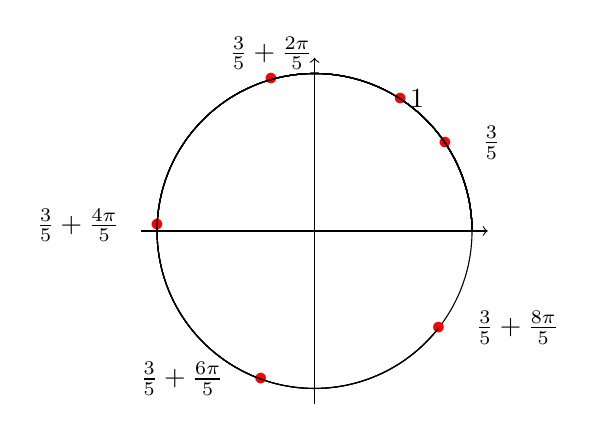
\begin{tikzpicture}[scale=2]
%Axes
\draw [->] (-1.1,0) -- (1.1,0);
\draw [->] (0,-1.1) -- (0,1.1);
%Cercle
\draw (0,0) circle (1);
%Points
\draw (1,0) arc (0:57:1) node [red] {$\bullet$};
\draw (1,0) arc (0:57:1) node[right] {$\ddp 1$} ;
\draw (1,0) arc (0:34:1) node [red] {$\bullet$};
\draw (1,0) arc (0:34:1) node[right] {$\quad \ddp \frac{3}{5}$} ;
\draw (1,0) arc (0:106:1) node [red] {$\bullet$};
\draw (1,0) arc (0:106:1) node[above] {$\ddp \frac{3}{5} + \frac{2\pi}{5}$} ;
\draw (1,0) arc (0:178:1) node [red] {$\bullet$};
\draw (1,0) arc (0:178:1) node[left] {$\ddp \frac{3}{5} + \frac{4\pi}{5}\quad$} ;
\draw (1,0) arc (0:250:1) node [red] {$\bullet$};
\draw (1,0) arc (0:250:1) node[left] {$\ddp \frac{3}{5} + \frac{6\pi}{5}\quad$} ;
\draw (1,0) arc (0:322:1) node [red] {$\bullet$};
\draw (1,0) arc (0:322:1) node[right] {$\quad \ddp \frac{3}{5} + \frac{8\pi}{5}$} ;
\end{tikzpicture}
\end{center}
\end{minipage}
%--------------------------------------------------
\item \textbf{R\'esolution de $\mathbf{\sin{\left(3x-\ddp\frac{\pi}{3}\right)}=\sin{\left(2x+\ddp\frac{\pi}{6}\right)}}$:}\\
\noindent De m\^{e}me, on sait que $\sin{(X)}=\sin{(Y)}\Leftrightarrow \left\lbrace\begin{array}{llll}  \exists k\in\Z,& X&=& Y+2k\pi\vsec\\ \hbox{ou}\vsec\\ \exists k\in\Z,& X&=& \pi-Y+2k\pi.    \end{array}\right.$ On peut appliquer cela ici et on obtient:
$$\sin{\left(3x-\ddp\frac{\pi}{3}\right)}=\sin{\left(2x+\ddp\frac{\pi}{6}\right)} \Leftrightarrow \left\lbrace\begin{array}{llll}  \exists k\in\Z,& 3x-\ddp\frac{\pi}{3}&=& 2x+\ddp\frac{\pi}{6}+2k\pi\vsec\\ \hbox{ou}\vsec\\ \exists k\in\Z,& 3x-\ddp\frac{\pi}{3}&=&\pi-2x-\ddp\frac{\pi}{6}+2k\pi    \end{array}\right. \Leftrightarrow \left\lbrace\begin{array}{llll}  \exists k\in\Z,& x&=& \ddp\frac{\pi}{2}+2k\pi\vsec\\ \hbox{ou}\vsec\\\exists k\in\Z,& x&=& \ddp\frac{7\pi}{30}+\ddp\frac{2k\pi}{5}.    \end{array}\right.$$
\begin{minipage}[c]{0.45\textwidth}
On obtient ainsi:
$$\fbox{$\mathcal{S}_{\R}=\left\lbrace \ddp\frac{\pi}{2}+2k\pi,\ k\in\Z\right\rbrace\cup\left\lbrace \ddp\frac{7\pi}{30}+\ddp\frac{2k\pi}{5},\ k\in\Z\right\rbrace$.}$$
Et on a :
$$\fbox{$\mathcal{S}_{[0,2\pi[}=\left\{ \ddp \frac{\pi}{2}, \frac{7\pi}{30}, \frac{19\pi}{30}, \frac{31\pi}{30}, \frac{43\pi}{30}, \frac{55\pi}{30}\right\}$}.$$
\end{minipage}
\quad \begin{minipage}[c]{0.45\textwidth}
\begin{center}
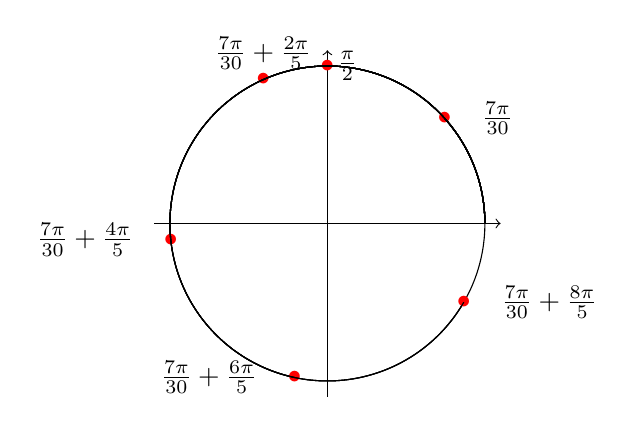
\begin{tikzpicture}[scale=2]
%Axes
\draw [->] (-1.1,0) -- (1.1,0);
\draw [->] (0,-1.1) -- (0,1.1);
%Cercle
\draw (0,0) circle (1);
%Points
\draw (1,0) arc (0:90:1) node [red] {$\bullet$};
\draw (1,0) arc (0:90:1) node[right] {$\ddp \frac{\pi}{2}$} ;
\draw (1,0) arc (0:42:1) node [red] {$\bullet$};
\draw (1,0) arc (0:42:1) node[right] {$\quad \ddp \frac{7\pi}{30}$} ;
\draw (1,0) arc (0:114:1) node [red] {$\bullet$};
\draw (1,0) arc (0:114:1) node[above] {$\ddp \frac{7\pi}{30} + \frac{2\pi}{5}$} ;
\draw (1,0) arc (0:186:1) node [red] {$\bullet$};
\draw (1,0) arc (0:186:1) node[left] {$\ddp \frac{7\pi}{30} + \frac{4\pi}{5}\quad$} ;
\draw (1,0) arc (0:258:1) node [red] {$\bullet$};
\draw (1,0) arc (0:258:1) node[left] {$\ddp \frac{7\pi}{30} + \frac{6\pi}{5}\quad$} ;
\draw (1,0) arc (0:330:1) node [red] {$\bullet$};
\draw (1,0) arc (0:330:1) node[right] {$\quad \ddp \frac{7\pi}{30} + \frac{8\pi}{5}$} ;
\end{tikzpicture}
\end{center}
\end{minipage}
%--------------------------------------------------
\item \textbf{R\'esolution de $\mathbf{\tan{(x+1)}+\tan{(3x+1)}=0}$:}
\begin{itemize}
\item[$\bullet$] On commence par rechercher le domaine de d\'efinition de cette \'equation. On doit donc avoir pour tout $k\in\Z$: $x+1\not= \ddp\frac{\pi}{2}+k\pi$ et $3x+1\not= \ddp\frac{\pi}{2}+k\pi$. On obtient donc que $\mathcal{D}=\R \setminus\left\lbrace  \ddp\frac{\pi}{2}-1+k\pi;\ddp\frac{\pi}{6}-\ddp\frac{1}{3}+\ddp\frac{k\pi}{3},\ k\in\Z  \right\rbrace$. 
\item[$\bullet$] De m\^{e}me que dans les deux exemples pr\'ec\'edents, on sait que $\tan{(X)}=\tan{(Y)}\Leftrightarrow \exists k\in\Z,\ X=Y+k\pi$. On peut appliquer cela ici et on obtient en utilisant tout d'abord l'imparit\'e de la tangente:
$$\begin{array}{lll} \tan{(x+1)}+\tan{(3x+1)}=0&\Leftrightarrow &\tan{(x+1)}=-\tan{(3x+1)} \Leftrightarrow  \tan{(x+1)}=\tan{(-3x-1)} \vsec\\
&\Leftrightarrow &\exists k\in\Z,\ x+1=-3x-1+k\pi\Leftrightarrow \exists k\in\Z,\ x=-\ddp\demi+\ddp\frac{k\pi}{4}.\end{array}$$
\end{itemize}
\begin{minipage}[c]{0.45\textwidth}
Comme pour tout $k\in\Z:$ $-\ddp\demi+\ddp\frac{k\pi}{4}\in\mathcal{D}$, on obtient:
$$\fbox{$\mathcal{S}_{\R}=\left\lbrace -\ddp\demi+\ddp\frac{k\pi}{4},\ k\in\Z\right\rbrace$}.$$
Et on a :
$$\fbox{$\mathcal{S}_{[0,2\pi[}=\left\{ - \ddp\frac{1}{2}, - \ddp\frac{1}{2}+\ddp\frac{\pi}{4},  - \ddp\frac{1}{2}+\ddp\frac{\pi}{2},  - \ddp\frac{1}{2}+\ddp\frac{3\pi}{4} \right\}$}.$$
\end{minipage}
\quad \begin{minipage}[c]{0.45\textwidth}
\begin{center}
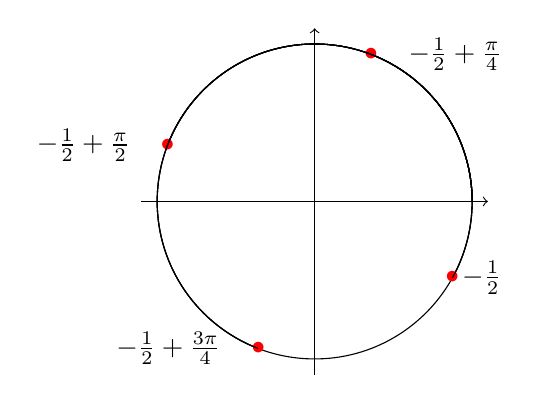
\begin{tikzpicture}[scale=2]
%Axes
\draw [->] (-1.1,0) -- (1.1,0);
\draw [->] (0,-1.1) -- (0,1.1);
%Cercle
\draw (0,0) circle (1);
%Points
\draw (1,0) arc (0:-29:1) node [red] {$\bullet$};
\draw (1,0) arc (0:-29:1) node[right] {$\ddp - \frac{1}{2}$} ;
\draw (1,0) arc (0:69:1) node [red] {$\bullet$};
\draw (1,0) arc (0:69:1) node[right] {$\quad \ddp - \ddp\frac{1}{2}+\ddp\frac{\pi}{4}$} ;
\draw (1,0) arc (0:159:1) node [red] {$\bullet$};
\draw (1,0) arc (0:159:1) node[left] {$\ddp - \ddp\frac{1}{2}+\ddp\frac{\pi}{2}\quad$} ;
\draw (1,0) arc (0:249:1) node [red] {$\bullet$};
\draw (1,0) arc (0:249:1) node[left] {$\ddp - \ddp\frac{1}{2}+\ddp\frac{3\pi}{4} \quad$} ;
\end{tikzpicture}
\end{center}
\end{minipage}
%--------------------------------------------------
\item \textbf{R\'esolution de $\mathbf{\sin^2{x}=\ddp\demi}$:}\\
\noindent  En posant $X=\sin{(x)}$, on doit r\'esoudre $X^2=\ddp\demi$, \`{a} savoir: $X=\ddp\frac{1}{\sqrt{2}}$ ou $X=-\ddp\frac{1}{\sqrt{2}}$. On doit donc r\'esoudre $\sin{(x)}=\ddp\frac{1}{\sqrt{2}}$ ou $\sin{(x)}=-\ddp\frac{1}{\sqrt{2}}$. On obtient ainsi
$$\fbox{$\mathcal{S}_{\R}=\left\lbrace  -\ddp\frac{3\pi}{4}+2k\pi,\ k\in\Z \right\rbrace \cup\left\lbrace  -\ddp\frac{\pi}{4}+2k\pi,\ k\in\Z \right\rbrace \cup\left\lbrace  \ddp\frac{\pi}{4}+2k\pi,\ k\in\Z \right\rbrace \cup\left\lbrace  \ddp\frac{3\pi}{4}+2k\pi,\ k\in\Z \right\rbrace$}$$
\begin{minipage}[c]{0.45\textwidth}
Et on a :
$$\fbox{$ \mathcal{S}_{\lbrack 0,2\pi\lbrack}=\left\lbrace \ddp\frac{\pi}{4},\ddp\frac{3\pi}{4},\ddp\frac{5\pi}{4},\ddp\frac{7\pi}{4}  \right\rbrace$}.$$
\end{minipage}
\quad \begin{minipage}[c]{0.45\textwidth}
\begin{center}
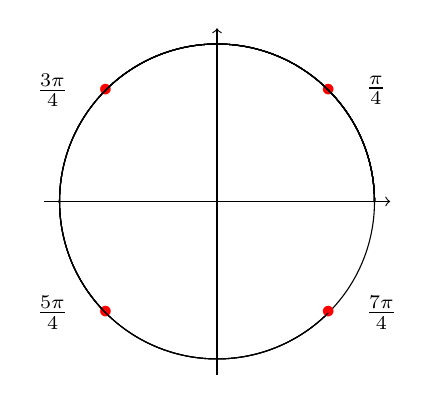
\begin{tikzpicture}[scale=2]
%Axes
\draw [->] (-1.1,0) -- (1.1,0);
\draw [->] (0,-1.1) -- (0,1.1);
%Cercle
\draw (0,0) circle (1);
%Points
\draw (1,0) arc (0:45:1) node [red] {$\bullet$};
\draw (1,0) arc (0:45:1) node[right] {$\quad\ddp \frac{\pi}{4}$} ;
\draw (1,0) arc (0:135:1) node [red] {$\bullet$};
\draw (1,0) arc (0:135:1) node[left] {$\ddp \ddp\frac{3\pi}{4}\quad$} ;
\draw (1,0) arc (0:225:1) node [red] {$\bullet$};
\draw (1,0) arc (0:225:1) node[left] {$\ddp \ddp\frac{5\pi}{4}\quad$} ;
\draw (1,0) arc (0:315:1) node [red] {$\bullet$};
\draw (1,0) arc (0:315:1) node[right] {$\quad \ddp \ddp\frac{7\pi}{4}$} ;
\end{tikzpicture}
\end{center}
\end{minipage}
%--------------------------------------------------
\item \textbf{R\'esolution de $\mathbf{\sin{(2x)}=\cos{\left(\ddp\frac{x}{2}\right)}}$:}\\
\noindent Une fa\c{c}on de faire ici est de transformer le cosinus en sinus. On obtient ainsi
$$\begin{array}{lll}\sin{(2x)}=\cos{\left(\ddp\frac{x}{2}\right)} &\Leftrightarrow &\sin{(2x)}=\sin{\left(\ddp\frac{\pi}{2}+\ddp\frac{x}{2}\right)} \Leftrightarrow \left\lbrace\begin{array}{llll}  \exists k\in\Z,& 2x&=& \ddp\frac{\pi}{2}+\ddp\frac{x}{2}+2k\pi\vsec\\ \hbox{ou}\vsec\\ \exists k\in\Z,& 2x&=&\pi-\ddp\frac{\pi}{2}-\ddp\frac{x}{2}+2k\pi    \end{array}\right. \vsec\\
&\Leftrightarrow & \left\lbrace\begin{array}{llll}  \exists k\in\Z,& x&=& \ddp\frac{\pi}{3}+\ddp\frac{4k\pi}{3}\vsec\\ \hbox{ou}\vsec\\ \exists k\in\Z,& x&=& \ddp\frac{\pi}{5}+\ddp\frac{4k\pi}{5}.    \end{array}\right.\end{array}$$
 \begin{minipage}[c]{0.45\textwidth}
On obtient ainsi:
$$\fbox{$\mathcal{S}_{\R}=\left\lbrace  \ddp\frac{\pi}{3}+\ddp\frac{4k\pi}{3} ,\ k\in\Z\right\rbrace\cup\left\lbrace  \ddp\frac{\pi}{5}+\ddp\frac{4k\pi}{5},\ k\in\Z\right\rbrace$}.$$
Et on a :
$$\fbox{$\mathcal{S}_{\lbrack 0,2\pi\lbrack}=\left\lbrace 
\ddp\frac{\pi}{5},\ddp\frac{\pi}{3},\ddp\frac{3\pi}{5},\ddp\frac{7\pi}{5},\pi,\ddp\frac{5\pi}{3},\ddp\frac{9\pi}{5}\right\rbrace$}.$$
\end{minipage}
\quad \begin{minipage}[c]{0.45\textwidth}
\begin{center}
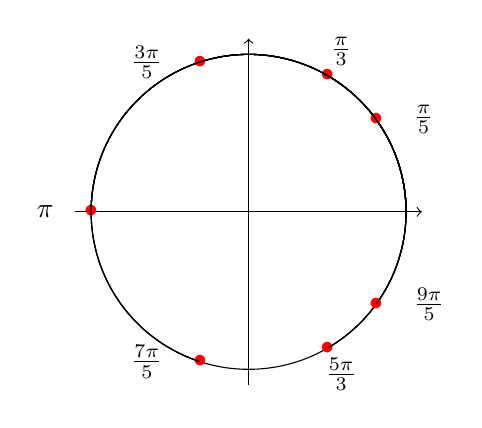
\begin{tikzpicture}[scale=2]
%Axes
\draw [->] (-1.1,0) -- (1.1,0);
\draw [->] (0,-1.1) -- (0,1.1);
%Cercle
\draw (0,0) circle (1);
%Points
\draw (1,0) arc (0:60:1) node [red] {$\bullet$};
\draw (1,0) arc (0:60:1) node[above] {$\quad\ddp \frac{\pi}{3}$} ;
\draw (1,0) arc (0:180:1) node [red] {$\bullet$};
\draw (1,0) arc (0:180:1) node[left] {$\ddp \pi \quad$} ;
\draw (1,0) arc (0:-60:1) node [red] {$\bullet$};
\draw (1,0) arc (0:-60:1) node[below] {$\quad \ddp \ddp\frac{5\pi}{3}$} ;
\draw (1,0) arc (0:36:1) node [red] {$\bullet$};
\draw (1,0) arc (0:36:1) node[right] {$\quad \ddp \ddp\frac{\pi}{5}$} ;
\draw (1,0) arc (0:108:1) node [red] {$\bullet$};
\draw (1,0) arc (0:108:1) node[left] {$ \ddp \ddp\frac{3\pi}{5} \quad$} ;
\draw (1,0) arc (0:252:1) node [red] {$\bullet$};
\draw (1,0) arc (0:252:1) node[left] {$ \ddp \ddp\frac{7\pi}{5}\quad$} ;
\draw (1,0) arc (0:-36:1) node [red] {$\bullet$};
\draw (1,0) arc (0:-36:1) node[right] {$\quad \ddp \ddp\frac{9\pi}{5}$} ;
\end{tikzpicture}
\end{center}
\end{minipage}
%--------------------------------------------------
\item \textbf{R\'esolution de $\mathbf{ 2\cos^2{(3x)}+3\cos{(3x)}+1=0    }$:}\\
\noindent On pose le changement de variable $X=\cos{(3x)}$ et on doit donc r\'esoudre $2X^2+3X+1=0$. Le discriminant vaut $\Delta=1$ et les deux solutions distinctes sont donc $X_1=-1$ et $X_2=-\ddp\demi$. Ainsi on doit donc r\'esoudre $\cos{(3x)}=-1$ et $\cos{(3x)}=-\ddp\demi$. La r\'esolution de ces deux \'equations fondamentales donne 
$$ \fbox{$\mathcal{S}_{\R}=\left\lbrace  \ddp\frac{\pi}{3}+\ddp\frac{2k\pi}{3} ,\ k\in\Z\right\rbrace\cup\left\lbrace  \ddp\frac{2\pi}{9}+\ddp\frac{2k\pi}{3},\ k\in\Z\right\rbrace\cup\left\lbrace  -\ddp\frac{2\pi}{9}+\ddp\frac{2k\pi}{3},\ k\in\Z\right\rbrace$}.$$
\begin{minipage}[c]{0.45\textwidth}
Et on a :
$$ \fbox{$\mathcal{S}_{\lbrack 0,2\pi\lbrack}=\left\lbrace \ddp\frac{2\pi}{9} , \ddp\frac{\pi}{3},\ddp\frac{4\pi}{9} ,\ddp\frac{8\pi}{9},\pi,\ddp\frac{10\pi}{9},\ddp\frac{14\pi}{9},\ddp\frac{5\pi}{3},\ddp\frac{16\pi}{9} \right\rbrace .$}$$
\end{minipage}
\quad \begin{minipage}[c]{0.45\textwidth}
\begin{center}
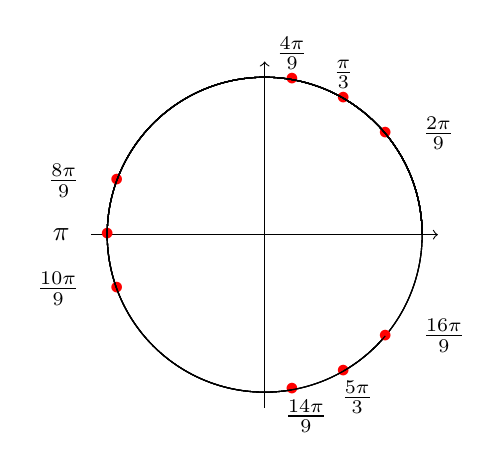
\begin{tikzpicture}[scale=2]
%Axes
\draw [->] (-1.1,0) -- (1.1,0);
\draw [->] (0,-1.1) -- (0,1.1);
%Cercle
\draw (0,0) circle (1);
%Points
\draw (1,0) arc (0:60:1) node [red] {$\bullet$};
\draw (1,0) arc (0:60:1) node[above] {$\ddp \frac{\pi}{3}$} ;
\draw (1,0) arc (0:180:1) node [red] {$\bullet$};
\draw (1,0) arc (0:180:1) node[left] {$\ddp \pi \quad$} ;
\draw (1,0) arc (0:-60:1) node [red] {$\bullet$};
\draw (1,0) arc (0:-60:1) node[below] {$\quad \ddp \ddp\frac{5\pi}{3}$} ;
\draw (1,0) arc (0:40:1) node [red] {$\bullet$};
\draw (1,0) arc (0:40:1) node[right] {$\quad \ddp \ddp\frac{2\pi}{9}$} ;
\draw (1,0) arc (0:80:1) node [red] {$\bullet$};
\draw (1,0) arc (0:80:1) node[above] {$ \ddp \ddp\frac{4\pi}{9}$} ;
\draw (1,0) arc (0:160:1) node [red] {$\bullet$};
\draw (1,0) arc (0:160:1) node[left] {$ \ddp \ddp\frac{8\pi}{9} \quad$} ;
\draw (1,0) arc (0:200:1) node [red] {$\bullet$};
\draw (1,0) arc (0:200:1) node[left] {$ \ddp \ddp\frac{10\pi}{9} \quad$} ;
\draw (1,0) arc (0:280:1) node [red] {$\bullet$};
\draw (1,0) arc (0:280:1) node[below] {$\quad \ddp \ddp\frac{14\pi}{9} $} ;
\draw (1,0) arc (0:320:1) node [red] {$\bullet$};
\draw (1,0) arc (0:320:1) node[right] {$\quad \ddp \ddp\frac{16\pi}{9} $} ;
\end{tikzpicture}
\end{center}
\end{minipage}
%--------------------------------------------------
%\item \textbf{R\'esolution de $\mathbf{\sin{x}+\ddp\frac{1}{\sqrt{3}}\cos{x}=-1}$:}\\
%\noindent M\^{e}me m\'ethode que dans l'exercice 3. On ne donne que la solution:
%\begin{equation*}
%\fbox{
%$\mathcal{S}_{\R}=\left\lbrace \ddp\frac{7\pi}{6}+2k\pi,\ k\in\Z  \right\rbrace\cup \left\lbrace -\ddp\frac{\pi}{2}+2k\pi,\ k\in\Z  \right\rbrace\ \hbox{et}\  \mathcal{S}_{\lbrack 0,2\pi\lbrack}=\left\lbrace \ddp\frac{7\pi}{6} , \ddp\frac{3\pi}{2}  \right\rbrace.$}
%\end{equation*}
%--------------------------------------------------
\item \textbf{R\'esolution de $\mathbf{2\sin^2{x}=\sqrt{3}\sin{(2x)} }$:}\\
\noindent En utilisant la formule de duplication du sinus, on obtient la factorisation suivante
$$\begin{array}{lll}
2\sin^2{x}=\sqrt{3}\sin{(2x)}& \Leftrightarrow& \sin{x}\left(\sin{x}-\sqrt{3}\cos{x} \right)=0\vsec\\
&\Leftrightarrow & \sin{x}=0\ \hbox{ou}\ \sin{x}-\sqrt{3}\cos{x}=0\vsec\\
&\Leftrightarrow & \exists k\in\Z,\  x=k\pi \ \hbox{ou}\ \sin{x}-\sqrt{3}\cos{x}=0.
\end{array}$$
La deuxi\`eme \'equation est de type $a\cos{x}+b\sin{x}$. On obtient :
$$\begin{array}{lll}
\sin{x}-\sqrt{3}\cos{x}&=&2\left( -\ddp\frac{\sqrt{3}}{2}\cos{x}+\frac{1}{2}\sin{x}   \right)
= 2\cos{\left(x-\ddp\frac{5\pi}{6}\right)}.
\end{array}$$
Ainsi,
$$\begin{array}{lll}
2\sin^2{x}=\sqrt{3}\sin{(2x)}& \Leftrightarrow& \exists k\in\Z,\  x=k\pi \ \hbox{ou}\ \cos{\left(x-\ddp\frac{5\pi}{6}\right)}=0
\Leftrightarrow \left\lbrace \begin{array}{llll}
\exists k\in\Z,&  x&=&k\pi\\
\hbox{ou}\\
\exists k\in\Z,&  x&=&\ddp\frac{4\pi}{3}+2k\pi\\
\hbox{ou}\\
\exists k\in\Z,& x&=&\ddp\frac{\pi}{3}+2k\pi\\
\end{array}\right.
\end{array}$$
On a donc :
$$\fbox{$\mathcal{S}_{\R}=\left\lbrace k\pi,\ k\in\Z  \right\rbrace\cup \left\lbrace \ddp\frac{4\pi}{3}+2k\pi,\ k\in\Z  \right\rbrace\cup \left\lbrace \ddp\frac{\pi}{3}+2k\pi,\ k\in\Z  \right\rbrace$}.$$
\begin{minipage}[c]{0.45\textwidth}
Et de plus :
$$\fbox{$\mathcal{S}_{\lbrack 0,2\pi\lbrack}=\left\lbrace 0,\ddp\frac{\pi}{3},\pi,\ddp\frac{4\pi}{3} \right\rbrace$}.$$
\end{minipage}
\quad \begin{minipage}[c]{0.45\textwidth}
\begin{center}
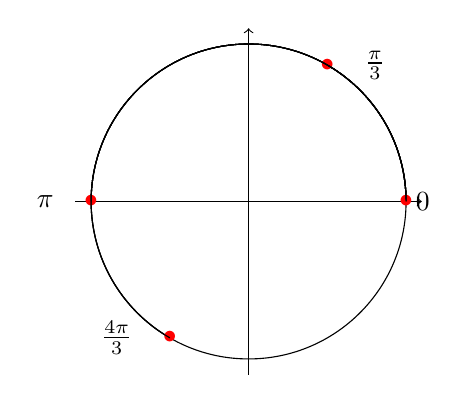
\begin{tikzpicture}[scale=2]
%Axes
\draw [->] (-1.1,0) -- (1.1,0);
\draw [->] (0,-1.1) -- (0,1.1);
%Cercle
\draw (0,0) circle (1);
%Points
\draw (1,0) arc (0:60:1) node [red] {$\bullet$};
\draw (1,0) arc (0:60:1) node[right] {$\quad \ddp \frac{\pi}{3}$} ;
\draw (1,0) arc (0:180:1) node [red] {$\bullet$};
\draw (1,0) arc (0:180:1) node[left] {$\ddp \pi \quad$} ;
\draw (1,0) arc (0:0:1) node [red] {$\bullet$};
\draw (1,0) arc (0:0:1) node[right] {$\ddp 0$} ;
\draw (1,0) arc (0:240:1) node [red] {$\bullet$};
\draw (1,0) arc (0:240:1) node[left] {$\ddp \ddp\frac{4\pi}{3}\quad$} ;
\end{tikzpicture}
\end{center}
\end{minipage}
%-----------------------------------
\item \textbf{R\'esolution de $\mathbf{ \sin{\left(2x-\ddp\frac{\pi}{4}\right)}=-\cos{\left(x+\ddp\frac{\pi}{6}\right)} }$:}\\
\noindent
On transforme le cosinus en sinus afin de se ramener \`a une \'equation fondamentale.
On a en utilisant l'imparit\'e du sinus:
$$
\sin{\left(2x-\ddp\frac{\pi}{4}\right)}=-\sin{\left(\ddp\frac{\pi}{2}-x-\frac{\pi}{6}\right)}
=\sin{\left(-\ddp\frac{\pi}{2}+x+\frac{\pi}{6}\right)}
=\sin{\left(x-\ddp\frac{\pi}{3}\right)}.$$
Ainsi,
$$
\sin{\left(2x-\ddp\frac{\pi}{4}\right)}=-\cos{\left(x+\ddp\frac{\pi}{6}\right)} \Leftrightarrow  \left\lbrace \begin{array}{l}
\exists k\in\Z,\ 2x-\ddp\frac{\pi}{4}=x-\ddp\frac{\pi}{3}+2k\pi\vsec\\
\hbox{ou}\vsec\\
\exists k\in\Z,\ 2x-\ddp\frac{\pi}{4}=\pi-x+\ddp\frac{\pi}{3}+2k\pi,
\end{array}\right.
\Leftrightarrow \left\lbrace\begin{array}{llll}
\exists k\in\Z, &x&=&-\ddp\frac{\pi}{12}+2k\pi\\
\hbox{ou}\\
\exists k\in\Z,& x&=&-\ddp\frac{5\pi}{36}+\frac{2k\pi}{3}.\\
\end{array}\right.$$
\begin{minipage}[c]{0.45\textwidth}
On obtient :
$$\fbox{$\mathcal{S}_{\R}=\left\lbrace -\ddp\frac{\pi}{12}+2k\pi,\ k\in\Z  \right\rbrace\cup \left\lbrace \ddp\frac{19\pi}{36}+\frac{2k\pi}{3},\ k\in\Z  \right\rbrace$}.$$ 
Et on a :
$$\fbox{$\mathcal{S}_{\lbrack 0,2\pi\lbrack}=\left\lbrace \ddp\frac{19\pi}{36}, \ddp\frac{43\pi}{36} ,\ddp\frac{67\pi}{36},\ddp\frac{23\pi}{12} \right\rbrace$}.$$
\end{minipage}
\quad \begin{minipage}[c]{0.45\textwidth}
\begin{center}
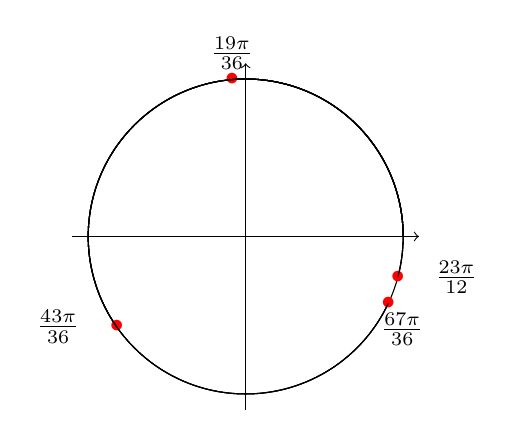
\begin{tikzpicture}[scale=2]
%Axes
\draw [->] (-1.1,0) -- (1.1,0);
\draw [->] (0,-1.1) -- (0,1.1);
%Cercle
\draw (0,0) circle (1);
%Points
\draw (1,0) arc (0:95:1) node [red] {$\bullet$};
\draw (1,0) arc (0:95:1) node[above] {$\ddp \frac{19\pi}{36}$} ;
\draw (1,0) arc (0:215:1) node [red] {$\bullet$};
\draw (1,0) arc (0:215:1) node[left] {$\ddp \frac{43\pi}{36} \quad$} ;
\draw (1,0) arc (0:335:1) node [red] {$\bullet$};
\draw (1,0) arc (0:335:1) node[below] {$\quad \ddp \frac{67\pi}{36}$} ;
\draw (1,0) arc (0:-15:1) node [red] {$\bullet$};
\draw (1,0) arc (0:-15:1) node[right] {$\quad\ddp \ddp\frac{23\pi}{12}$} ;
\end{tikzpicture}
\end{center}
\end{minipage}
%--------------------------------------------------
\item \textbf{R\'esolution de $\mathbf{\sqrt{3}\cos^2{x}+2\cos{x}\sin{x}-\sqrt{3}\sin^2{x}=\sqrt{2}}$:}\\
\noindent On commence par utiliser le formulaire de trigonom\'etrie afin de transformer l'expression:
$$\sqrt{3}\cos^2{x}+2\cos{x}\sin{x}-\sqrt{3}\sin^2{x}=\sqrt{3}\left(\cos^2{x}-\sin^2{x}  \right)+\sin{(2x)}=\sqrt{3}\cos{(2x)}+\sin{(2x)}.$$
On pose $X=2x$, et on factorise $\sqrt{3}\cos{(2x)}+\sin{(2x)}$. \\
\begin{minipage}[c]{0.45\textwidth}
On obtient :
$$\fbox{$\mathcal{S}_{\R}= \left\lbrace \ddp\frac{5\pi}{24}+k\pi,\ k\in\Z  \right\rbrace\cup \left\lbrace -\ddp\frac{\pi}{24}+k\pi,\ k\in\Z  \right\rbrace$}.$$
Et on a :
$$\fbox{$\mathcal{S}_{\lbrack 0,2\pi\lbrack}= \left\lbrace \ddp\frac{5\pi}{24},\ddp\frac{23\pi}{24},\ddp\frac{29\pi}{24},\ddp\frac{47\pi}{24}  \right\rbrace .$}$$
\end{minipage}
\quad \begin{minipage}[c]{0.45\textwidth}
\begin{center}
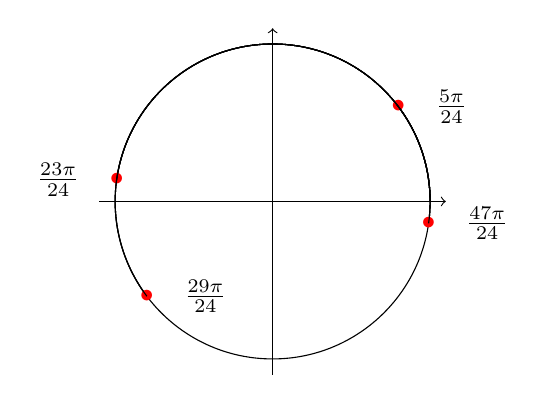
\begin{tikzpicture}[scale=2]
%Axes
\draw [->] (-1.1,0) -- (1.1,0);
\draw [->] (0,-1.1) -- (0,1.1);
%Cercle
\draw (0,0) circle (1);
%Points
\draw (1,0) arc (0:37:1) node [red] {$\bullet$};
\draw (1,0) arc (0:37:1) node[right] {$\quad \ddp \frac{5\pi}{24}$} ;
\draw (1,0) arc (0:-8:1) node [red] {$\bullet$};
\draw (1,0) arc (0:-8:1) node[right] {$\quad\ddp \frac{47\pi}{24} $} ;
\draw (1,0) arc (0:172:1) node [red] {$\bullet$};
\draw (1,0) arc (0:172:1) node[left] {$\ddp \frac{23\pi}{24}\quad $} ;
\draw (1,0) arc (0:217:1) node [red] {$\bullet$};
\draw (1,0) arc (0:217:1) node[right] {$\quad\ddp \ddp\frac{29\pi}{24}$} ;
\end{tikzpicture}
\end{center}
\end{minipage}
%--------------------------------------------------
\item \textbf{R\'esolution de $\mathbf{1+\cos{x}+\sin{(5x)}+\sin{(6x)}=0}$:}\\
\noindent On commence par transformer l'expression gr\^{a}ce au formulaire de trigonom\'etrie afin de la mettre sous forme factoris\'ee. On obtient
$$ 1+\cos{x}+\sin{(5x)}+\sin{(6x)}=2\cos^2{\left(  \ddp\frac{x}{2}\right)}+2\sin{\left(  \ddp\frac{11x}{2}\right)}\cos{\left(  \ddp\frac{x}{2}\right)}=2\cos{\left(  \ddp\frac{x}{2}\right)} \left(  \cos{\left(  \ddp\frac{x}{2}\right)}  +\sin{\left(  \ddp\frac{11x}{2}\right)} \right).$$
Ainsi r\'esoudre $1+\cos{x}+\sin{(5x)}+\sin{(6x)}=0$ est \'equivalent \`{a} r\'esoudre $\cos{\left(  \ddp\frac{x}{2}\right)}=0$ ou $\cos{\left(  \ddp\frac{x}{2}\right)}  +\sin{\left(  \ddp\frac{11x}{2}\right)} =0$. On peut d\'ej\`{a} r\'esoudre la premi\`{e}re \'equation et on obtient
$$ \cos{\left(  \ddp\frac{x}{2}\right)}=0 \Leftrightarrow\exists k\in\Z,\  \ddp\frac{x}{2}=\ddp\frac{\pi}{2}+k\pi\Leftrightarrow\exists k\in\Z,\  x=\pi+2k\pi.$$
\'Etudions la deuxi\`{e}me \'equation:
$$\hspace{-1cm} \begin{array}{lll}\cos{\left(  \ddp\frac{x}{2}\right)}  +\sin{\left(  \ddp\frac{11x}{2}\right)} =0 &\Leftrightarrow &\cos{\left(  \ddp\frac{x}{2}\right)} =-\sin{\left(  \ddp\frac{11x}{2}\right)} \Leftrightarrow \cos{\left(  \ddp\frac{x}{2}\right)} =\sin{\left( - \ddp\frac{11x}{2}\right)} \Leftrightarrow
\cos{\left(  \ddp\frac{x}{2}\right)} =\cos{\left(\ddp\frac{\pi}{2} + \ddp\frac{11x}{2}\right)}\vsec\\ &\Leftrightarrow&
\left\lbrace\begin{array}{lllll}
\exists k\in\Z, & \ddp\frac{x}{2}&=& \ddp\frac{\pi}{2} + \ddp\frac{11x}{2}+2k\pi\\
\hbox{ou}\\
\exists k\in\Z, & \ddp\frac{x}{2}&=& -\ddp\frac{\pi}{2} - \ddp\frac{11x}{2}+2k\pi
\end{array}\right. \Leftrightarrow \left\lbrace\begin{array}{lllll}
\exists k\in\Z, & x&=& -\ddp\frac{\pi}{10} - \ddp\frac{2k\pi}{5}\\
\hbox{ou}\\
\exists k\in\Z, & x&=& -\ddp\frac{\pi}{12} - \ddp\frac{k\pi}{3}.
\end{array}\right. \end{array}$$
Ainsi, on obtient 
\begin{equation*}
 \fbox{
 \begin{minipage}[t]{0.7\textwidth}
$\mathcal{S}=\left\lbrace  \pi+2k\pi,\ k\in\Z\right\rbrace\cup\left\lbrace   -\ddp\frac{\pi}{10} - \ddp\frac{2k\pi}{5}, \ k\in\Z\right\rbrace\cup\left\lbrace -\ddp\frac{\pi}{12} - \ddp\frac{k\pi}{3},\ k\in\Z\right\rbrace\\ \hbox{et}\  \mathcal{S}_{\lbrack 0,2\pi\lbrack}= \left\lbrace \ddp\frac{\pi}{4},\ddp\frac{3\pi}{10},\ddp\frac{7\pi}{12},\ddp\frac{7\pi}{10},\ddp\frac{11\pi}{12},\pi,\ddp\frac{11\pi}{10},\ddp\frac{15\pi}{12},\ddp\frac{15\pi}{10},\ddp\frac{19\pi}{12},\ddp\frac{19\pi}{10},\ddp\frac{23\pi}{12}            \right\rbrace.$
\end{minipage}}
\end{equation*}
%--------------------------------------------------
\item \textbf{R\'esolution de $\mathbf{\tan^4{x}+2\tan^2{x}-3=0}$:}\\
\noindent On pose le changement de variable $X=\tan^2{(x)}$ et on doit donc r\'esoudre: $X^2+2X-3=0$. Le calcul du discriminant donne que les solutions sont $-3$ et $1$. Ainsi, on doit r\'esoudre les deux \'equations $\tan^2{(x)}=-3$ et $\tan^2{(x)}=1$. Comme un carr\'e est toujours positif, la premi\`{e}re \'equation est impossible. La deuxi\`{e}me \'equation donne $\tan{(x)}=-1$ ou $\tan{(x)}=1$. \\
 \begin{minipage}[c]{0.45\textwidth}
On obtient donc
$$\fbox{$\mathcal{S}_{\R}=\left\lbrace -\ddp\frac{\pi}{4}+k\pi,\ k\in\Z \right\rbrace\cup\left\lbrace \ddp\frac{\pi}{4}+k\pi,\ k\in\Z \right\rbrace$}.$$
$$\fbox{$ \mathcal{S}_{\lbrack 0,2\pi\lbrack}= \left\lbrace \ddp\frac{\pi}{4},\ddp\frac{3\pi}{4},\ddp\frac{5\pi}{4},\ddp\frac{7\pi}{4}   \right\rbrace$}.$$
\end{minipage}
\quad \begin{minipage}[c]{0.45\textwidth}
\begin{center}
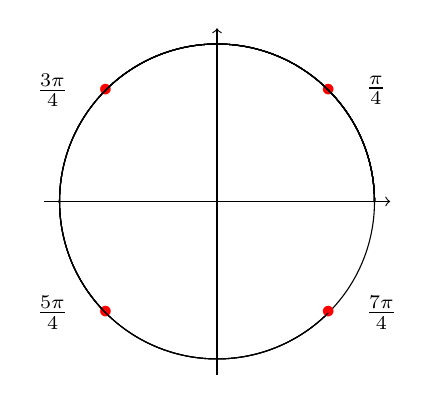
\begin{tikzpicture}[scale=2]
%Axes
\draw [->] (-1.1,0) -- (1.1,0);
\draw [->] (0,-1.1) -- (0,1.1);
%Cercle
\draw (0,0) circle (1);
%Points
\draw (1,0) arc (0:45:1) node [red] {$\bullet$};
\draw (1,0) arc (0:45:1) node[right] {$\quad\ddp \frac{\pi}{4}$} ;
\draw (1,0) arc (0:135:1) node [red] {$\bullet$};
\draw (1,0) arc (0:135:1) node[left] {$\ddp \ddp\frac{3\pi}{4}\quad$} ;
\draw (1,0) arc (0:225:1) node [red] {$\bullet$};
\draw (1,0) arc (0:225:1) node[left] {$\ddp \ddp\frac{5\pi}{4}\quad$} ;
\draw (1,0) arc (0:315:1) node [red] {$\bullet$};
\draw (1,0) arc (0:315:1) node[right] {$\quad \ddp \ddp\frac{7\pi}{4}$} ;
\end{tikzpicture}
\end{center}
\end{minipage}
\end{enumerate}
\end{correction}
%---------------------------------------------------
%--------------------------------------------------


%%---------------------------------------------------
%%--------------------------------------------------

%------------------------------------------------------------------------------------------
\begin{exercice}  \;
\begin{enumerate}
\item Soit $\ddp x \in \R\backslash \left\{ \pi + 2 k \pi, k \in \Z \right\}$. On pose : $u =  \tan \left(\ddp \frac{x}{2} \right).$ \'Etablir les relations suivantes, et indiquer pour quelles valeurs de $x$ elles sont valides :\\
\begin{minipage}[t]{0.3\textwidth}
(a) $\ddp \cos x = \frac{1-u^2}{1+u^2}$
\end{minipage}
\begin{minipage}[t]{0.3\textwidth}
(b)  $\ddp \sin x = \frac{2 u}{1+u^2}$
\end{minipage}
\begin{minipage}[t]{0.3\textwidth}
(c) $\ddp \tan x = \frac{2 u}{1-u^2}$
\end{minipage}
\item En utilisant ces relations, r\'esoudre sur $\R$ l'\'equation : $\ddp \cos x - 3 \sin x + 2\tan \left( \frac{x}{2} \right) - 1 = 0.$
\end{enumerate}
\end{exercice}
%------------------------------------------------------------------------------------------

\begin{correction}   \;
\begin{enumerate}
\item Tout d'abord, $u=\tan \left( \frac{x}{2}\right)$ est bien d\'efini pour $\ddp x \in \R\backslash \left\{ \pi + 2 k \pi, k \in \Z \right\}$.
\begin{itemize}
\item[(a)] On a $1+u^2>0$ donc $\ddp \frac{1-u^2}{1+u^2}$ est bien d\'efini. De plus, on a 
$$\frac{1-u^2}{1+u^2} = \frac{1-\frac{\sin^2 \left( \frac{x}{2}\right) }{\cos^2 \left( \frac{x}{2}\right) }}{1+\frac{\sin^2 \left( \frac{x}{2}\right) }{\cos^2 \left( \frac{x}{2}\right) }} = \frac{\cos^2 \left( \frac{x}{2}\right) - \sin^2 \left( \frac{x}{2}\right)}{\cos^2 \left( \frac{x}{2}\right) + \sin^2 \left( \frac{x}{2}\right)} = \frac{\cos x}{1} = \cos x.$$
\item[(b)] De m\^eme, $1+u^2>0$ donc $\ddp \frac{2 u}{1+u^2}$ est bien d\'efini. De plus, on a 
$$\frac{2 u}{1+u^2} = \frac{ 2 \frac{\sin \left( \frac{x}{2}\right) }{\cos \left( \frac{x}{2}\right) }}{1+\frac{\sin^2 \left( \frac{x}{2}\right) }{\cos^2 \left( \frac{x}{2}\right) }} = \frac{ 2 \cos \left( \frac{x}{2}\right) \sin \left( \frac{x}{2}\right)}{\cos^2 \left( \frac{x}{2}\right) + \sin^2 \left( \frac{x}{2}\right)} = \frac{\sin x}{1} = \sin x.$$
\item[(c)] On a $1-u^2 \not=0$ si et seulement si $\ddp \tan^2 \left( \frac{x}{2}\right) \not=1$, c'est-\`a-dire $\ddp \tan \left( \frac{x}{2}\right) \not\in \{-1,1\}$. On doit donc avoir $x \in \ddp \R\backslash \left( \left\{ \pi + 2 k \pi, k \in \Z \right\} \cup \left\{ \frac{\pi}{2} + k \pi, k \in \Z \right\} \right)$. On a alors :
$$\frac{2 u}{1- u^2} = \frac{ 2 \frac{\sin \left( \frac{x}{2}\right) }{\cos \left( \frac{x}{2}\right) }}{1-\frac{\sin^2 \left( \frac{x}{2}\right) }{\cos^2 \left( \frac{x}{2}\right) }} = \frac{ 2 \cos \left( \frac{x}{2}\right) \sin \left( \frac{x}{2}\right)}{\cos^2 \left( \frac{x}{2}\right) - \sin^2 \left( \frac{x}{2}\right)} = \frac{\sin x}{\cos x} = \tan x.$$
 \end{itemize}
\item L'\'equation est d\'efinie pour $\ddp \frac{x}{2} \in \R\backslash \left\{ \frac{\pi}{2} + k \pi, k \in \Z \right\}$. Le domaine de d\'efinition est donc  \conclusion{$\mathcal{D}=\ddp \R\backslash \left\{ \pi + 2 k \pi, k \in \Z \right\}$}.\\
On pose alors $u =  \tan \left(\ddp \frac{x}{2} \right)$, et on utilise les formules de la question pr\'ec\'edentes pour transformer l'\'equation. On est ramen\'es \`a r\'esoudre
$$\frac{1-u^2}{1+u^2} - 3 \frac{2u}{1+u^2} + 2u - 1 = 0 \Leftrightarrow \frac{1-u^2- 6u + 2u +2u^3-1-u^2}{1+u^2} = 0   \Leftrightarrow \frac{2u(u^2-u-2)}{1+u^2}  = 0.$$
On doit donc trouver les $u$ tels que le num\'erateur s'annule. On obtient $u \in \{0,-1, 2\}$. On doit ensuite revenir \`a la variable $x$, on r\'esout donc 
\begin{itemize}
\item[$\bullet$] $\tan\left( \ddp \frac{x}{2} \right) = 0 \Leftrightarrow \frac{x}{2} = k \pi, k \in \Z \Leftrightarrow  x = 2k\pi, k \in \Z$ 
\item[$\bullet$] $\tan\left( \ddp \frac{x}{2} \right) = -1\Leftrightarrow \frac{x}{2} = - \frac{\pi}{4} + k \pi, k \in \Z \Leftrightarrow  x = - \frac{\pi}{2} +2k\pi, k \in \Z$ 
\item[$\bullet$] $\tan\left( \ddp \frac{x}{2} \right) = 2 \Leftrightarrow \frac{x}{2} = \arctan(2) + k \pi, k \in \Z \Leftrightarrow  x = \arctan(2)  +2k\pi, k \in \Z$.
\end{itemize}
$$\fbox{ $ S = \ddp \left\{2 k \pi, k \in \Z \right\} \cup  \left\{-\frac{\pi}{2} + 2 k\pi, k \in \Z \right\} \cup \left\{2\arctan 2 + 2 k \pi, k \in \Z \right\} $}$$
\end{enumerate}
\end{correction}






%\newpage
%------------------------------------------------
%-------------------------------------------------
%-------------------------------------------------
%--------------------------------------------------
%----------------------------------------------------------------------------------------------
%-----------------------------------------------------------------------------------------------



\begin{exercice}   \;
R\'esoudre les in\'equations suivantes dans $\R$, puis dans $\lbrack 0,2\pi\lbrack$ et $\rbrack -\pi,\pi\rbrack$ :
\begin{enumerate}
\begin{minipage}[t]{0.45\textwidth}
\item $2\sin{x}-1<0$
\item $2\cos{(2x)}>\sqrt{3}$
\item $\ddp\frac{1}{\sqrt{3}}\tan{(3x)}>1$
\end{minipage}
\begin{minipage}[t]{0.45\textwidth}
\item $\sin{(3x)}\geq -\ddp\frac{\sqrt{3}}{2}$
\item $\sqrt{2}\cos{(3x)}\leq 1$
\item $\tan{(x)}\leq 1$
\end{minipage}
\end{enumerate}
\end{exercice}

\begin{correction}   \;
\begin{enumerate}
%------------------------------
\item \textbf{R\'esolution de $\mathbf{2\sin{(x)}-1<0}$:}  On se ram\`ene \`a une in\'equation fondamentale :$2\sin{x}-1<0  \Leftrightarrow \sin{x}<\ddp\frac{1}{2}.$\\
On r\'esout alors cette in\'equation fondamentale graphiquement:\\
\begin{minipage}[c]{0.45\textwidth}
\fbox{$ \mathcal{S}_{\R}= \ddp \mathop{\bigcup}\limits_{k\in \Z} \left] - \frac{7\pi}{6} + 2k\pi , \frac{\pi}{6} + 2k \pi \right[$}.\\
Et on a : \conclusion{$\mathcal{S}_{\lbrack 0,2\pi\lbrack}=\left\lbrack 0,\ddp\frac{\pi}{6}\right\lbrack\cup\left\rbrack \ddp\frac{5\pi}{6},2\pi\right\lbrack$}.\\
Et finalement : \conclusion{$ \mathcal{S}_{\rbrack -\pi,\pi\rbrack}=\left\rbrack -\pi,\ddp\frac{\pi}{6}\right\lbrack\cup\left\rbrack \ddp\frac{5\pi}{6},\pi\right\rbrack.$}
\end{minipage}
\quad 
\begin{center}
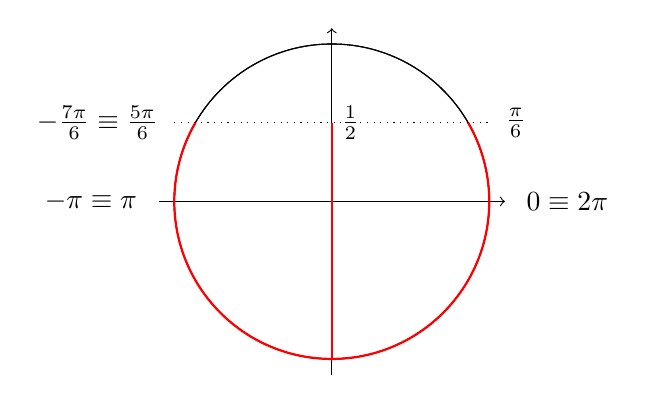
\begin{tikzpicture}[scale=2]
%Axes
\draw [->] (-1.1,0) -- (1.1,0);
\draw [->] (0,-1.1) -- (0,1.1);
%Cercle
\draw (0,0) circle (1);
%Intervalles axes
\draw [red,{-[}, thick] (0,-1) -- (0,0.5) ;
%Traits
\draw [dotted] (-1,0.5) -- (1,0.5) ;
%Points
\draw (0,0.5) node[right] {$\ddp \frac{1}{2}$};
\draw (1,0) arc (0:-210:1) node[left] {$\ddp - \frac{7\pi}{6} \equiv \frac{5\pi}{6} \quad $} ;
\draw (1,0) arc (0:30:1) node[right] {$\quad \ddp \frac{\pi}{6}$} ;
\draw (1,0) arc (0:0:1) node[right] {$\quad 0 \equiv 2\pi$} ;
\draw (1,0) arc (0:180:1) node[left] {$ -\pi \equiv \pi \quad$} ;
%Intervalles cercle
\draw [red, {-[}, thick] (1,0) arc (0:30:1) ;
\draw [red, {-[}, thick] (1,0) arc (0:-210:1) ;
\end{tikzpicture}
\end{center}

%------------------------------
\item \textbf{R\'esolution de $\mathbf{2\cos{(2x)}>\sqrt{3}}$:} On se ram\`ene \`a une in\'equation fondamentale :
$$2\cos{(2x)}>\sqrt{3}  \Leftrightarrow \cos{(2x)}>\ddp\frac{\sqrt{3}}{2}\quad (\star).$$
\begin{minipage}[c]{0.45\textwidth}
On r\'esout alors cette in\'equation fondamentale graphiquement:\\
$$\begin{array}{lll}
(\star) & \Leftrightarrow & \exists k\in\Z,\ -\ddp\frac{\pi}{6}+2k\pi <  2x < \ddp\frac{\pi}{6}+2k\pi\vsec\\
&\Leftrightarrow & \exists k\in\Z,\ -\ddp\frac{\pi}{12}+k\pi <  x < \ddp\frac{\pi}{12}+k\pi.
\end{array}$$
\end{minipage}
\quad \begin{minipage}[c]{0.45\textwidth}
\begin{center}
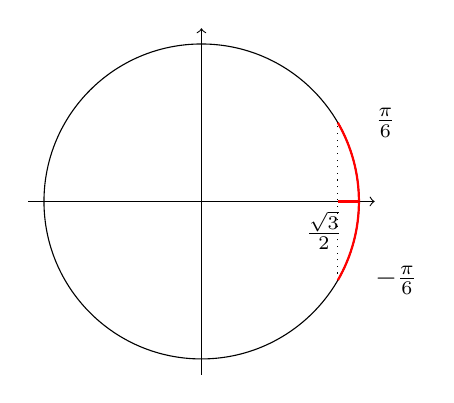
\begin{tikzpicture}[scale=2]
%Axes
\draw [->] (-1.1,0) -- (1.1,0);
\draw [->] (0,-1.1) -- (0,1.1);
%Cercle
\draw (0,0) circle (1);
%Intervalles axes
\draw [red,{]-}, thick] (0.866,0) -- (1,0) ;
%Traits
\draw [dotted] (0.866,-0.5) -- (0.866,0.5) ;
%Points
\draw (0.866,0) node[left, below] {$\ddp \frac{\sqrt{3}}{2} \quad$};
\draw (1,0) arc (0:-30:1) node[right] {$\quad \ddp - \frac{\pi}{6} $} ;
\draw (1,0) arc (0:30:1) node[right] {$\quad \ddp \frac{\pi}{6}$} ;
%Intervalles cercle
\draw [red, {-[}, thick] (1,0) arc (0:30:1) ;
\draw [red, {-[}, thick] (1,0) arc (0:-30:1) ;
\end{tikzpicture}
\end{center}
\end{minipage}
On obtient donc : $\fbox{$ \mathcal{S}_{\R}= \ddp \mathop{\bigcup}\limits_{k\in \Z} \left] - \frac{\pi}{12} + k\pi , \frac{\pi}{12} + k \pi \right[$}.$\\
Bien penser \`a refaire un deuxi\`eme cercle pour tracer les solutions, et pouvoir en d\'eduire les solutions sur les intervalles demand\'es. \\
\begin{minipage}[c]{0.45\textwidth}
On a :
$$\fbox{$\mathcal{S}_{\lbrack 0,2\pi\lbrack}=\left\lbrack 0,\ddp\frac{\pi}{12}\right\lbrack\cup\left\rbrack \ddp\frac{11\pi}{12},\ddp\frac{13\pi}{12}\right\lbrack\cup\left\rbrack \ddp\frac{23\pi}{12},2\pi\right\lbrack$}.$$
Et finalement :
 $$\fbox{$\mathcal{S}_{\rbrack -\pi,\pi\rbrack}=\left\rbrack -\pi,-\ddp\frac{11\pi}{12}\right\lbrack\cup\left\rbrack -\ddp\frac{\pi}{12},\ddp\frac{\pi}{12}\right\lbrack\cup\left\rbrack \ddp\frac{11\pi}{12},\pi\right\rbrack.$}$$
 \end{minipage}
\quad \begin{minipage}[c]{0.45\textwidth}
\begin{center}
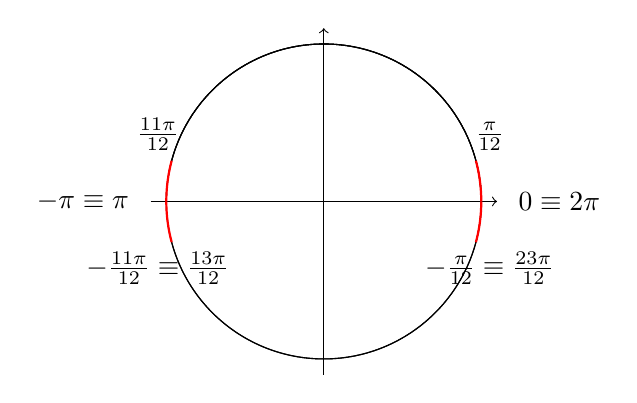
\begin{tikzpicture}[scale=2]
%Axes
\draw [->] (-1.1,0) -- (1.1,0);
\draw [->] (0,-1.1) -- (0,1.1);
%Cercle
\draw (0,0) circle (1);
%Points
\draw (1,0) arc (0:15:1) node[above] {$\quad \ddp \frac{\pi}{12}$} ;
\draw (1,0) arc (0:-15:1) node[below] {$\quad \ddp -\frac{\pi}{12} \equiv \frac{23\pi}{12}$} ;
\draw (1,0) arc (0:165:1) node[above] {$ \ddp \frac{11\pi}{12}\quad$} ;
\draw (1,0) arc (0:-165:1) node[below] {$\ddp -\frac{11\pi}{12} \equiv \frac{13\pi}{12}\quad$} ;
\draw (1,0) arc (0:0:1) node[right] {$\quad 0 \equiv 2\pi$} ;
\draw (1,0) arc (0:180:1) node[left] {$ -\pi \equiv \pi \quad$} ;
%Intervalles cercle
\draw [red, {-[}, thick] (1,0) arc (0:-15:1) ;
\draw [red, {-[}, thick] (1,0) arc (0:15:1) ;
\draw [red, {-[}, thick] (-1,0) arc (180:165:1) ;
\draw [red, {-[}, thick] (-1,0) arc (180:195:1) ;
\end{tikzpicture}
\end{center}
\end{minipage}
%-----------------------------
\item \textbf{R\'esolution de $\mathbf{\ddp\frac{1}{\sqrt{3}}\tan{(3x)>1 }}$:} On se ram\`ene \`a une in\'equation fondamentale :
$$\ddp\frac{1}{\sqrt{3}}\tan{(3x)}>1  \Leftrightarrow \tan{(3x)}>\sqrt{3}\quad (\star)$$
\begin{minipage}[c]{0.45\textwidth}
On r\'esout alors cette in\'equation fondamentale graphiquement:\\
$$\begin{array}{lll}
(\star)&\Leftrightarrow & \exists k\in\Z,\ \ddp\frac{\pi}{3}+k\pi <  3x < \ddp\frac{\pi}{2}+k\pi\vsec\\
&\Leftrightarrow & \exists k\in\Z,\ \ddp\frac{\pi}{9}+\ddp\frac{k\pi}{3} <  x < \ddp\frac{\pi}{6}+\ddp\frac{k\pi}{3}.
\end{array}$$
On obtient :
%$$\fbox{$ \mathcal{S}_{\R}=\left\lbrace x\in\R,\ \exists k\in\Z,\   \ddp\frac{\pi}{9}+\ddp\frac{k\pi}{3} <  x < \ddp\frac{\pi}{6}+\ddp\frac{k\pi}{3}\right\rbrace.$}$$
$$\fbox{$ \mathcal{S}_{\R}= \ddp \mathop{\bigcup}\limits_{k\in \Z} \left] \frac{\pi}{9} + \frac{k\pi}{3} , \frac{\pi}{6} + \frac{k \pi}{3} \right[$}.$$
\end{minipage}
\quad \begin{minipage}[c]{0.45\textwidth}
\begin{center}
\begin{tikzpicture}[scale=2]
%Axes
\draw [->] (-1.1,0) -- (1.1,0);
\draw [->] (0,-1.1) -- (0,1.1);
\draw (1,-1.1) -- (1,2);
%Cercle
\draw (0,0) circle (1);
%Intervalles axes
\draw [red,{]-}, thick] (1,1.732) -- (1,2);
%Traits
\draw [dotted] (0,0) -- (1,1.732) ;
%Points
\draw (1,1.732) node[right] {$\quad \ddp \sqrt{3}$};
\draw (1,0) arc (0:90:1) node[above] {$\quad \ddp \frac{\pi}{2} $} ;
\draw (1,0) arc (0:60:1) node[right] {$\quad \ddp \frac{\pi}{3}$} ;
%Intervalles cercle
\draw [red, {]-[}, thick] (0,1) arc (90:60:1) ;
\end{tikzpicture}
\end{center}
\end{minipage}
On refait alors un autre cercle trigonom\'etrique (\`{a} faire) afin de placer les angles solutions et on obtient, en prenant $k\in\intent{ 0,5}$ : \conclusion{$\mathcal{S}_{\lbrack 0,2\pi\lbrack}=\left\rbrack \ddp\frac{\pi}{9},\ddp\frac{\pi}{6} \right\lbrack\cup\left\rbrack \ddp\frac{4\pi}{9},\ddp\frac{\pi}{2} \right\lbrack\cup\left\rbrack \ddp\frac{7\pi}{9},\ddp\frac{5\pi}{6} \right\lbrack\cup\left\rbrack \ddp\frac{10\pi}{9},\ddp\frac{7\pi}{6} \right\lbrack\cup\left\rbrack \ddp\frac{13\pi}{9},\ddp\frac{3\pi}{2} \right\lbrack\cup\left\rbrack \ddp\frac{16\pi}{9},\ddp\frac{11\pi}{6} \right\lbrack .$}
Enfin, on a : \conclusion{$\ddp \mathcal{S}_{]-\pi,\pi]}=\left]-\frac{8\pi}{9}, -\frac{5\pi}{6} \right[ \cup \left] - \frac{5\pi}{9}, - \frac{\pi}{2}\right[ \cup \left] -\frac{\pi}{3}, -\frac{\pi}{6}\right[ \cup \left\rbrack \ddp\frac{\pi}{9},\ddp\frac{\pi}{6} \right\lbrack\cup \left\rbrack \ddp\frac{4\pi}{9},\ddp\frac{\pi}{2} \right\lbrack \cup \left\rbrack \ddp\frac{7\pi}{9},\ddp\frac{5\pi}{6} \right\lbrack$}.
%------------------------------
\item \textbf{R\'esolution de $\mathbf{ \sin{(3x)} \geq -\ddp\frac{\sqrt{3}}{2}}$:}\\
\begin{minipage}[c]{0.45\textwidth}
\noindent  La r\'esolution graphique sur le cercle trigonom\'etrique donne: 
$$\begin{array}{rcl}
\ddp \sin{(3x)}\geq -\ddp\frac{\sqrt{3}}{2} & \Leftrightarrow & \ddp \exists k\in\Z,\ -\ddp\frac{\pi}{3}+2k\pi\leq 3x\leq \ddp\frac{4\pi}{3}+2k\pi\vsec\\
&  \Leftrightarrow & \ddp \exists k\in\Z,\ -\ddp\frac{\pi}{9}+\frac{2k\pi}{3} \leq x \leq \ddp\frac{4\pi}{9}+\frac{2k\pi}{3}
\end{array} $$
On obtient donc : 
$$\fbox{$ \mathcal{S}_{\R}= \ddp \mathop{\bigcup}\limits_{k\in \Z} \left[ -\frac{\pi}{9} + \frac{2 k\pi}{3} , \frac{4\pi}{9} + \frac{2k \pi}{3} \right]$}.$$
\end{minipage}
%quad \begin{minipage}[c]{0.45\textwidth}
\begin{center}
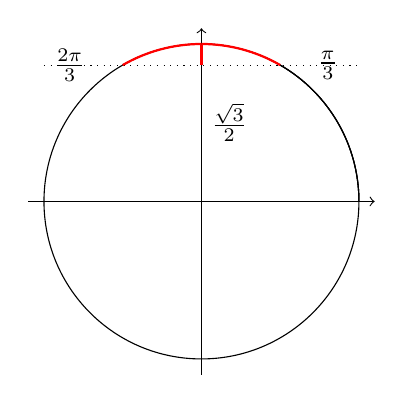
\begin{tikzpicture}[scale=2]
%Axes
\draw [->] (-1.1,0) -- (1.1,0);
\draw [->] (0,-1.1) -- (0,1.1);
%Cercle
\draw (0,0) circle (1);
%Intervalles axes
\draw [red,{[-}, thick] (0,0.866) -- (0,1) ;
%Traits
\draw [dotted] (-1,0.866) -- (1,0.866) ;
%Points
\draw (0,0.5) node[right] {$\ddp \frac{\sqrt{3}}{2}$};
\draw (1,0) arc (0:120:1) node[left] {$\ddp \frac{2\pi}{3} \quad $} ;
\draw (1,0) arc (0:60:1) node[right] {$\quad \ddp \frac{\pi}{3}$} ;
%Intervalles cercle
\draw [red, {-]}, thick] (0,1) arc (90:60:1) ;
\draw [red, {-]}, thick] (0,1) arc (90:120:1) ;
\end{tikzpicture}
\end{center}

On fait un cercle trigonom\'etrique pour placer les solutions, et on obtient, en prenant $k \in \intent{ 0, 2 }$ :
$$ \fbox{$\mathcal{S}_{\lbrack 0,2\pi\lbrack}=\left\lbrack 0,\ddp\frac{4\pi}{9} \right\rbrack\cup\left\lbrack \ddp\frac{5\pi}{9},\ddp\frac{10\pi}{9} \right\rbrack\cup\left\lbrack \ddp\frac{11\pi}{9},\ddp\frac{16\pi}{9} \right\rbrack\cup\left\lbrack \ddp\frac{17\pi}{9},2\pi \right\lbrack$}.$$
Et finalement :
$$ \fbox{$\mathcal{S}_{\rbrack -\pi,\pi\rbrack}=\left\rbrack -\pi,-\ddp\frac{8\pi}{9} \right\rbrack\cup\left\lbrack -\ddp\frac{7\pi}{9},-\ddp\frac{2\pi}{9} \right\rbrack\cup\left\lbrack -\ddp\frac{\pi}{9},\ddp\frac{4\pi}{9} \right\rbrack\cup\left\lbrack \ddp\frac{5\pi}{9},\pi \right\rbrack$}.$$
%------------------------------
\newpage
\item \textbf{R\'esolution de $\mathbf{ \sqrt{2}\cos{(3x)}\leq 1 }$:}\\
\noindent On a: $ \sqrt{2}\cos{(3x)}\leq 1 \Leftrightarrow \cos{(3x)}\leq \ddp\frac{1}{\sqrt{2}}$. \\
\begin{minipage}[c]{0.45\textwidth}
La r\'esolution sur le cercle trigonom\'etrique donne : 
$$\begin{array}{rcl}
\cos{(3x)}\leq \ddp\frac{1}{\sqrt{2}} & \Leftrightarrow& \ddp \exists k\in\Z,\ \ddp\frac{\pi}{4}+2k\pi\leq 3x\leq \ddp\frac{7\pi}{4}+2k\pi\vsec\\
&\Leftrightarrow& \ddp  \exists k\in\Z,\ \ddp\frac{\pi}{12}+\ddp\frac{2k\pi}{3}\leq 3x\leq \ddp\frac{7\pi}{12}+\ddp\frac{2k\pi}{3}
\end{array}$$ 
On obtient donc : 
$$\fbox{$ \mathcal{S}_{\R}= \ddp \mathop{\bigcup}\limits_{k\in \Z} \left[ \frac{\pi}{12} + \frac{2 k\pi}{3} , \frac{7\pi}{12} + \frac{2k \pi}{3} \right]$}.$$
\end{minipage}
\quad \begin{minipage}[c]{0.45\textwidth}
\begin{center}
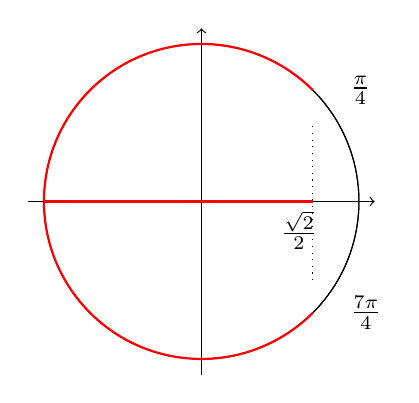
\begin{tikzpicture}[scale=2]
%Axes
\draw [->] (-1.1,0) -- (1.1,0);
\draw [->] (0,-1.1) -- (0,1.1);
%Cercle
\draw (0,0) circle (1);
%Intervalles axes
\draw [red,{-]}, thick] (-1,0) -- (0.707,0)  ;
%Traits
\draw [dotted] (0.707,-0.5) -- (0.707,0.5) ;
%Points
\draw (0.707,0) node[left, below] {$\ddp \frac{\sqrt{2}}{2} \quad$};
\draw (1,0) arc (0:-45:1) node[right] {$\quad \ddp \frac{7\pi}{4} $} ;
\draw (1,0) arc (0:45:1) node[right] {$\quad \ddp \frac{\pi}{4}$} ;
%Intervalles cercle
\draw [red, {-]}, thick] (-1,0) arc (180:45:1) ;
\draw [red, {-]}, thick] (-1,0) arc (-180:-45:1) ;
\end{tikzpicture}
\end{center}
\end{minipage}
Afin de donner les solutions dans $\lbrack 0,2\pi\lbrack$ et dans $\rbrack -\pi,\pi\rbrack$, on repr\'esente les solutions sur un cercle trigonom\'etrique en prenant $k=0,\ k=1$ et $k=2$. On obtient alors:
$$\fbox{$\mathcal{S}_{\lbrack 0,2\pi\lbrack}=\left\lbrack \ddp\frac{\pi}{12},\ddp\frac{7\pi}{12} \right\rbrack\cup\left\lbrack \ddp\frac{9\pi}{12},\ddp\frac{15\pi}{12} \right\rbrack\cup\left\lbrack \ddp\frac{17\pi}{12},\ddp\frac{23\pi}{12} \right\rbrack$}.$$
Et finalement :
$$\fbox{$ \mathcal{S}_{\rbrack -\pi,\pi\rbrack}=\left\rbrack -\pi,-\ddp\frac{9\pi}{12}  \right\rbrack\cup\left\lbrack -\ddp\frac{7\pi}{12},-\ddp\frac{\pi}{12} \right\rbrack\cup\left\lbrack \ddp\frac{\pi}{12},\ddp\frac{7\pi}{12} \right\rbrack\cup\left\lbrack \ddp\frac{9\pi}{12},\pi\right\rbrack$}.$$
%------------------------------
\item \textbf{R\'esolution de $\mathbf{ \tan{(x)}\leq 1 }$:}\\
\begin{minipage}[c]{0.45\textwidth}
\noindent La r\'esolution graphique sur le cercle trigonom\'etrique  donne :
$$\tan{(x)}\leq 1 \Leftrightarrow \exists k\in\Z,\ -\ddp\frac{\pi}{2}+k\pi < x\leq \ddp\frac{\pi}{4}+k\pi.$$
On obtient : \fbox{$ \mathcal{S}_{\R}= \ddp \mathop{\bigcup}\limits_{k\in \Z} \left] - \frac{\pi}{2} + k\pi, \frac{\pi}{4} + k \pi \right]$}.
\end{minipage}
\quad \begin{minipage}[c]{0.45\textwidth}
\begin{center}
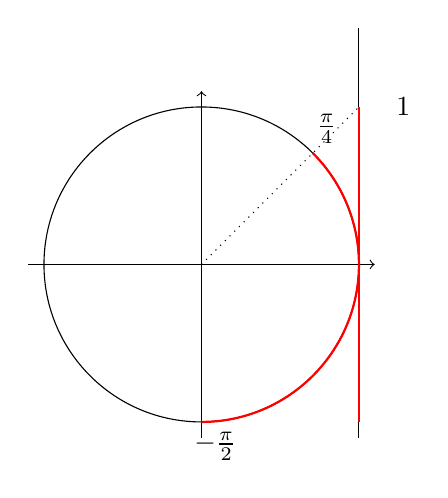
\begin{tikzpicture}[scale=2]
%Axes
\draw [->] (-1.1,0) -- (1.1,0);
\draw [->] (0,-1.1) -- (0,1.1);
\draw (1,-1.1) -- (1,1.5);
%Cercle
\draw (0,0) circle (1);
%Intervalles axes
\draw [red,{-]}, thick] (1,-1) -- (1,1);
%Traits
\draw [dotted] (0,0) -- (1,1) ;
%Points
\draw (1,1) node[right] {$\quad \ddp 1$};
\draw (1,0) arc (0:-90:1) node[below] {$\quad \ddp - \frac{\pi}{2} $} ;
\draw (1,0) arc (0:45:1) node[above] {$\quad \ddp \frac{\pi}{4}$} ;
%Intervalles cercle
\draw [red, {-]}, thick] (1,0) arc (0:45:1) ;
\draw [red, {-[}, thick] (1,0) arc (0:-90:1) ;
\end{tikzpicture}
\end{center}
\end{minipage}
Attention, les solutions pour la tangente sont d\'efinies modulo $\pi$, et non $2\pi$. Il y a donc deux intervalles solutions \`a tracer sur le cercle trigonom\'etrique.\\
\begin{minipage}[c]{0.45\textwidth}
On a donc : \fbox{$\mathcal{S}_{\lbrack 0,2\pi\lbrack}=\left\lbrack 0,\ddp\frac{\pi}{4}  \right\rbrack\cup \left\rbrack \ddp\frac{\pi}{2},\ddp\frac{5\pi}{4}  \right\rbrack\cup\left\rbrack \ddp\frac{3\pi}{2},2\pi  \right\lbrack$}.\\
Et finalement : \fbox{$ \mathcal{S}_{\rbrack -\pi,\pi\rbrack}=\left\rbrack -\pi,-\ddp\frac{3\pi}{4}  \right\rbrack\cup
\left\rbrack -\ddp\frac{\pi}{2},\ddp\frac{\pi}{4}  \right\rbrack\cup\left\rbrack \ddp\frac{\pi}{2},\pi  \right\rbrack
$}.
\end{minipage}
\quad \begin{minipage}[c]{0.45\textwidth}
\begin{center}
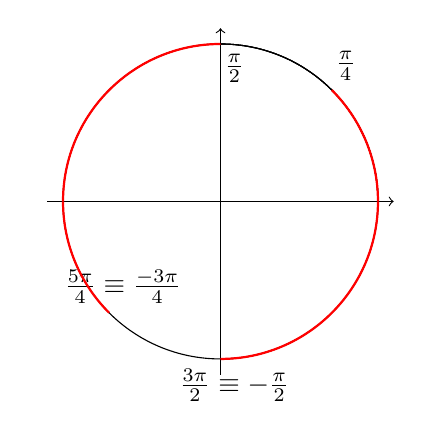
\begin{tikzpicture}[scale=2]
%Axes
\draw [->] (-1.1,0) -- (1.1,0);
\draw [->] (0,-1.1) -- (0,1.1);
%Cercle
\draw (0,0) circle (1);
%Points
\draw (1,0) arc (0:-90:1) node[below] {$\quad \ddp \frac{3\pi}{2} \equiv - \frac{\pi}{2}$} ;
\draw (1,0) arc (0:45:1) node[above] {$\quad \ddp \frac{\pi}{4}$} ;
\draw (1,0) arc (0:90:1) node[below] {$\quad \ddp  \frac{\pi}{2} $} ;
\draw (1,0) arc (0:225:1) node[above] {$\quad \ddp \frac{5\pi}{4} \equiv \frac{-3\pi}{4}$} ;
%Intervalles cercle
\draw [red, {-]}, thick] (1,0) arc (0:45:1) ;
\draw [red, {-[}, thick] (1,0) arc (0:-90:1) ;
\draw [red, {-[}, thick] (-1,0) arc (180:90:1) ;
\draw [red, {-]}, thick] (-1,0) arc (180:225:1) ;
\end{tikzpicture}
\end{center}
\end{minipage}
%------------------------------
\end{enumerate}
\end{correction}


%------------------------------------------------
%-------------------------------------------------
\begin{exercice}  \;
R\'esoudre sur $\R$ les in\'equations suivantes et repr\'esenter l'ensemble des solutions sur le cercle trigonom\'etrique:
\begin{enumerate}
\begin{minipage}[t]{0.45\textwidth}
\item $4\sin^2{x}-(2+2\sqrt{3})\sin{x}+\sqrt{3}\leq 0$
\item $\tan^2{x}-1<0$
\item $2\cos^2{(3x)}-3\cos{(3x)}+1\leq 0$   
\item $\tan^2{x}-(\sqrt{3}-1)\tan{x}-\sqrt{3}<0$
\item $\ddp\frac{1}{4}\leq \sin^2{x}\leq \ddp\demi$
\end{minipage}
\begin{minipage}[t]{0.45\textwidth}
\item $\cos{(x)}-\sin{(x)}\geq \ddp\frac{\sqrt{6}}{2}$  
\item $\sin{(x)}-\ddp\frac{1}{\sqrt{3}}\cos{(x)}\leq -1$
\item $\cos{x}+\sin{x}-1<0$
\item $\sqrt{3}\cos{x}+\sin{x}-\sqrt{2}<0$
\end{minipage}
\end{enumerate}
\end{exercice}
\begin{correction}    \;
\begin{enumerate}
%------------------------------
\item \textbf{R\'esolution de $\mathbf{4\sin^2{(x)}-(2+2\sqrt{3})\sin{(x)}+\sqrt{3}\leq 0     }$:}\\
\noindent On pose $X=\sin{(x)}$ et on doit donc r\'esoudre $4X^2-(2+2\sqrt{3})X+\sqrt{3}\leq 0$. Le calcul du discriminant donne $\Delta=(2\sqrt{3}-2)^2$ et on obtient ainsi comme solutions $\ddp\frac{\sqrt{3}}{2}$ et $\ddp\demi$. 
Ainsi :
$$4X^2-(2+2\sqrt{3})X+\sqrt{3}\leq 0 \Leftrightarrow \ddp\demi\leq X\leq \ddp\frac{\sqrt{3}}{2}.$$ 
Comme $X=\sin{(x)}$, on obtient au final que: 
$$4\sin^2{(x)}-(2+2\sqrt{3})\sin{(x)}+\sqrt{3}\leq 0\Leftrightarrow  \ddp\demi\leq \sin{(x)}\leq \ddp\frac{\sqrt{3}}{2}.$$
\begin{minipage}[c]{0.45\textwidth}
La r\'esolution sur le cercle trigonom\'etrique donne
%$$\fbox{$\mathcal{S}_{\R}=\left\lbrace \ddp\frac{\pi}{6}+2k\pi\leq x\leq \ddp\frac{\pi}{3}+2k\pi,\ k\in\Z \right\rbrace\cup\left\lbrace  \ddp\frac{2\pi}{3}+2k\pi\leq x\leq \ddp\frac{5\pi}{6}+2k\pi,\ k\in\Z  \right\rbrace$.}$$
$$\fbox{$\mathcal{S}_{\R}= \ddp \mathop{\bigcup}\limits_{k\in \Z}  \left( \left[ \ddp\frac{\pi}{6}+2k\pi , \ddp\frac{\pi}{3}+2k\pi \right] \cup \left[  \ddp\frac{2\pi}{3}+2k\pi , \ddp\frac{5\pi}{6}+2k\pi\right] \right)$.}$$
\end{minipage}
%\quad \begin{minipage}[c]{0.45\textwidth}
\begin{center}
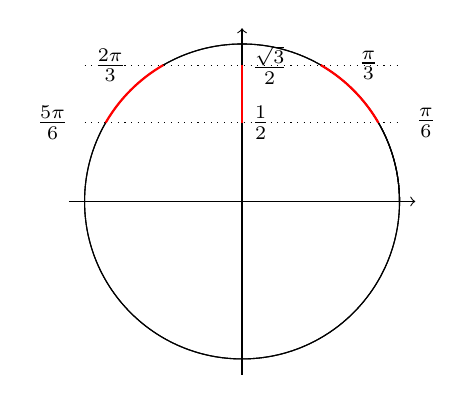
\begin{tikzpicture}[scale=2]
%Axes
\draw [->] (-1.1,0) -- (1.1,0);
\draw [->] (0,-1.1) -- (0,1.1);
%Cercle
\draw (0,0) circle (1);
%Intervalles axes
\draw [red,{[-]}, thick] (0,0.5) -- (0,0.866) ;
%Traits
\draw [dotted] (-1,0.5) -- (1,0.5) ;
\draw [dotted] (-1,0.866) -- (1,0.866) ;
%Points
\draw (0,0.866) node[right] {$\ddp \frac{\sqrt{3}}{2}$};
\draw (0,0.5) node[right] {$\ddp \frac{1}{2}$};
\draw (1,0) arc (0:-210:1) node[left] {$\ddp  \frac{5\pi}{6} \quad $} ;
\draw (1,0) arc (0:30:1) node[right] {$\quad \ddp \frac{\pi}{6}$} ;
\draw (1,0) arc (0:60:1) node[right] {$\quad \ddp \frac{\pi}{3}$} ;
\draw (1,0) arc (0:120:1) node[left] {$\ddp \frac{2\pi}{3}\quad $} ;
%Intervalles cercle
\draw [red, {[-]}, thick] (0.866,0.5) arc (30:60:1) ;
\draw [red, {[-]}, thick] (-0.866,0.5) arc (150:120:1) ;
\end{tikzpicture}
\end{center}
%\end{minipage}
%------------------------------
\item \textbf{R\'esolution de $\mathbf{\tan^2{(x)}-1<0    }$:}\\
\noindent On a: $\tan^2{x}-1<0 \Leftrightarrow -1<\tan{(x)}<1$. La r\'esolution graphique sur le cercle trigonom\'etrique (\`a faire) donne
$$\fbox{$\mathcal{S}_{\R}= \mathop{\bigcup}\limits_{k\in \Z}  \left] -\ddp\frac{\pi}{4}+k\pi , \ddp\frac{\pi}{4}+k\pi \right[$}.$$
%------------------------------
\item \textbf{R\'esolution de $\mathbf{2\cos^2{(3x)}-3\cos{(3x)}+1\leq 0    }$:}\\
\noindent On pose $X=\cos{(3x)}$ et on doit donc r\'esoudre $2X^2-3X+1\leq 0$. 
Le calcul du discriminant donne que les solutions sont $\ddp\demi$ et 1. 
Ainsi $2X^2-3X+1\leq 0 \Leftrightarrow \ddp\demi\leq X\leq 1$. Comme $X=\cos{(3x)}$, on obtient que: $$2\cos^2{(3x)}-3\cos{(3x)}+1\leq 0\Leftrightarrow  \ddp\demi\leq \cos{(3x)}\leq 1.$$ 
\begin{minipage}[c]{0.45\textwidth}
La r\'esolution sur le cercle trigonom\'etrique donne :
$$\ddp\demi\leq \cos{(3x)}\leq 1 \Leftrightarrow \exists k \in \Z, -\ddp\frac{\pi}{3}+2k\pi\leq x\leq \ddp\frac{\pi}{3}+2k\pi.$$
\end{minipage}
\quad \begin{minipage}[c]{0.45\textwidth}
\begin{center}
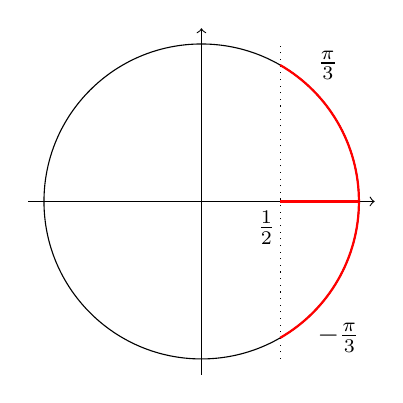
\begin{tikzpicture}[scale=2]
%Axes
\draw [->] (-1.1,0) -- (1.1,0);
\draw [->] (0,-1.1) -- (0,1.1);
%Cercle
\draw (0,0) circle (1);
%Intervalles axes
\draw [red,{]-}, thick] (0.5,0) -- (1,0) ;
%Traits
\draw [dotted] (0.5,-1) -- (0.5,1) ;
%Points
\draw (0.5,0) node[left, below] {$\ddp \frac{1}{2} \quad$};
\draw (1,0) arc (0:-60:1) node[right] {$\quad \ddp - \frac{\pi}{3} $} ;
\draw (1,0) arc (0:60:1) node[right] {$\quad \ddp \frac{\pi}{3}$} ;
%Intervalles cercle
\draw [red, {-[}, thick] (1,0) arc (0:60:1) ;
\draw [red, {-[}, thick] (1,0) arc (0:-60:1) ;
\end{tikzpicture}
\end{center}
\end{minipage}\\
\begin{minipage}[c]{0.45\textwidth}
On obtient donc :
$$\fbox{$\mathcal{S}_{\R}= \ddp \mathop{\bigcup}\limits_{k\in \Z} \left[ -\ddp\frac{\pi}{9}+\ddp\frac{2k\pi}{3}, \ddp\frac{\pi}{9}+\ddp\frac{2k\pi}{3} \right[$}.$$
\end{minipage}
\quad \begin{minipage}[c]{0.45\textwidth}
\begin{center}
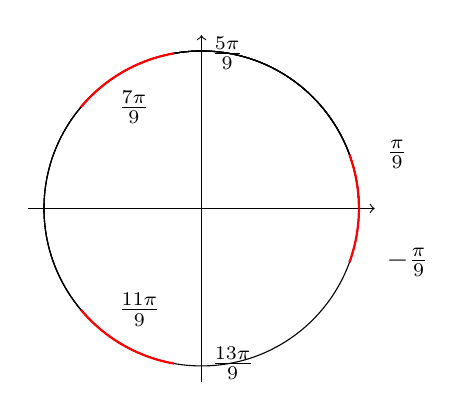
\begin{tikzpicture}[scale=2]
%Axes
\draw [->] (-1.1,0) -- (1.1,0);
\draw [->] (0,-1.1) -- (0,1.1);
%Cercle
\draw (0,0) circle (1);
%Points
\draw (1,0) arc (0:-20:1) node[right] {$\quad \ddp - \frac{\pi}{9} $} ;
\draw (1,0) arc (0:20:1) node[right] {$\quad \ddp \frac{\pi}{9}$} ;
\draw (1,0) arc (0:100:1) node[right] {$\quad \ddp \frac{5\pi}{9} $} ;
\draw (1,0) arc (0:140:1) node[right] {$\quad \ddp \frac{7\pi}{9}$} ;
\draw (1,0) arc (0:220:1) node[right] {$\quad \ddp \frac{11\pi}{9} $} ;
\draw (1,0) arc (0:260:1) node[right] {$\quad \ddp \frac{13\pi}{9}$} ;
%Intervalles cercle
\draw [red, {-]}, thick] (1,0) arc (0:-20:1) ;
\draw [red, {-]}, thick] (1,0) arc (0:20:1) ;
\draw [red, {[-]}, thick] (-0.174,0.985) arc (100:140:1) ;
\draw [red, {[-]}, thick] (-0.766,-0.643) arc (220:260:1) ;
\end{tikzpicture}
\end{center}
\end{minipage}
%------------------------------
\item \textbf{R\'esolution de $\mathbf{\tan^2{(x)}-(\sqrt{3}-1)\tan{(x)}-\sqrt{3}<0    }$:}\\
\noindent On pose $X=\tan{(x)}$ et on doit donc r\'esoudre $X^2-(\sqrt{3}-1)X-\sqrt{3}<0$. Le discriminant vaut $\Delta=(1+\sqrt{3})^2$ et ainsi les solutions sont $-1$ et $\sqrt{3}$. On obtient donc :
$$X^2-(\sqrt{3}-1)X-\sqrt{3}<0 \Leftrightarrow -1<X<\sqrt{3}.$$ 
Comme $X=\tan{(x)}$, on obtient que: 
$$\tan^2{(x)}-(\sqrt{3}-1)\tan{(x)}-\sqrt{3}<0 \Leftrightarrow -1<\tan{(x)}<\sqrt{3}.$$ 
La r\'esolution par le cercle trigonom\'etrique (\`a faire) donne
$$\fbox{$\mathcal{S}_{\R}=\ddp \mathop{\bigcup}\limits_{k\in \Z}  \left] -\ddp\frac{\pi}{4}+k\pi,  \ddp\frac{\pi}{3}+k\pi\right[$}.$$
%------------------------------
\item \textbf{R\'esolution de $\mathbf{\ddp\frac{1}{4}\leq \sin^2{(x)}\leq \ddp\demi   }$:}\\
\noindent On pose $X=\sin{(x)}$ et on doit r\'esoudre $\ddp\frac{1}{4}\leq X^2\leq \ddp\demi$ ce qui est \'equivalent \`{a} $X^2- \ddp\demi\leq 0$ et $\ddp\frac{1}{4}- X^2\leq 0$. Comme 
$X^2- \ddp\demi\leq 0\Leftrightarrow -\ddp\frac{1}{\sqrt{2}}\leq X\leq \ddp\frac{1}{\sqrt{2}}$ et que $\ddp\frac{1}{4}- X^2\leq 0 \Leftrightarrow X\geq \ddp\demi\ \hbox{ou}\ X\leq -\ddp\demi$, on obtient que
$$ \ddp\frac{1}{4}\leq X^2\leq \ddp\demi \Leftrightarrow X\in\left\lbrack -\ddp\frac{1}{\sqrt{2}}, -\ddp\frac{1}{2}\right\rbrack\cup \left\lbrack \ddp\frac{1}{2}, \ddp\frac{1}{\sqrt{2}}\right\rbrack\Leftrightarrow \sin{(x)}\in\left\lbrack -\ddp\frac{1}{\sqrt{2}}, -\ddp\frac{1}{2}\right\rbrack\cup \left\lbrack \ddp\frac{1}{2}, \ddp\frac{1}{\sqrt{2}}\right\rbrack.$$ 
La r\'esolution sur le cercle trigonom\'etrique (\`a faire) donne 
$$\fbox{$\mathcal{S}= \ddp \mathop{\bigcup}\limits_{k\in \Z} \left[ -\ddp\frac{5\pi}{6}+2k\pi, -\ddp\frac{3\pi}{4}+2k\pi \right] \cup \left[ -\ddp\frac{\pi}{4}+2k\pi, -\ddp\frac{\pi}{6}+2k\pi \right] \cup \left[ \ddp\frac{\pi}{6}+2k\pi,  \ddp\frac{\pi}{4}+2k\pi \right] \cup\left[ \ddp\frac{3\pi}{4}+2k\pi, \ddp\frac{5\pi}{6}+2k\pi\right]$}.$$
%------------------------------
\item \textbf{R\'esolution de $\mathbf{\cos{(x)}-\sin{(x)}\geq \ddp\frac{\sqrt{6}}{2}   }$:}\\
\noindent On reconna\^{i}t la forme $a\cos{(x)}+b\sin{(x)}$ et on obtient donc
$$\cos{(x)}-\sin{(x)}\geq \ddp\frac{\sqrt{6}}{2} \Leftrightarrow \sqrt{2}\left( \ddp\frac{1}{\sqrt{2}} \cos{(x)}-\ddp\frac{1}{\sqrt{2}}\sin{(x)}  \right)\geq \ddp\frac{\sqrt{6}}{2}\Leftrightarrow \cos{\left(x  +\ddp\frac{\pi}{4} \right)}\geq \ddp\frac{\sqrt{3}}{2}.$$
On a ainsi obtenu une in\'egalit\'e fondamentale de type $\cos{(X)}\geq \ddp\frac{\sqrt{3}}{2}$ (avec ici $X=x+\ddp\frac{\pi}{4}$) et on r\'esout donc cela graphiquement sur le cercle trigonom\'etrique (\`a faire). On obtient alors
$$\cos{\left(x  +\ddp\frac{\pi}{4} \right)}\geq \ddp\frac{\sqrt{3}}{2} \Leftrightarrow \exists k\in\Z,\ -\ddp\frac{\pi}{6}+2k\pi\leq x+\ddp\frac{\pi}{4}\leq \ddp\frac{\pi}{6}+2k\pi\Leftrightarrow  \exists k\in\Z,\ -\ddp\frac{5\pi}{12}+2k\pi\leq x\leq -\ddp\frac{\pi}{12}+2k\pi.$$
On obtient donc les solutions suivantes:
$$\fbox{$\mathcal{S}_{\R}= \ddp \mathop{\bigcup}\limits_{k\in \Z} \left[  -\ddp\frac{5\pi}{12}+2k\pi, -\ddp\frac{\pi}{12}+2k\pi \right]$}.$$
%------------------------------
\item \textbf{R\'esolution de $\mathbf{\sin{(x)}-\ddp\frac{1}{\sqrt{3}}\cos{(x)}\leq -1}$:}\\
\noindent On reconna\^{i}t la forme $a\cos{(x)}+b\sin{(x)}$ et on obtient donc
$$\sin{(x)}-\ddp\frac{1}{\sqrt{3}}\cos{(x)}\leq -1 \Leftrightarrow -\ddp\frac{2}{\sqrt{3}}\left( \ddp\demi \cos{(x)}-\ddp\frac{\sqrt{3}}{2}\sin{(x)}  \right)\leq -1\Leftrightarrow \cos{\left(x  +\ddp\frac{\pi}{3} \right)}\geq \ddp\frac{\sqrt{3}}{2}.$$
On a chang\'e le sens de l'in\'egalit\'e car $-\ddp\frac{2}{\sqrt{3}}<0$. On a ainsi obtenu une in\'egalit\'e fondamentale de type $\cos{(X)}\geq \ddp\frac{\sqrt{3}}{2}$ (avec ici $X=x+\ddp\frac{\pi}{3}$) et on r\'esout donc cela graphiquement sur le cercle trigonom\'etrique (\`a faire). On obtient alors
$$\cos{\left(x  +\ddp\frac{\pi}{3} \right)}\geq \ddp\frac{\sqrt{3}}{2} \Leftrightarrow \exists k\in\Z,\ -\ddp\frac{\pi}{6}+2k\pi\leq x+\ddp\frac{\pi}{3}\leq \ddp\frac{\pi}{6}+2k\pi\Leftrightarrow  \exists k\in\Z,\ -\ddp\frac{\pi}{2}+2k\pi\leq x\leq -\ddp\frac{\pi}{6}+2k\pi.$$
On obtient donc les solutions suivantes:
$$\fbox{$\mathcal{S}_{\R}=\ddp \mathop{\bigcup}\limits_{k\in \Z} \left[  -\ddp\frac{\pi}{2}+2k\pi, -\ddp\frac{\pi}{6}+2k\pi \right]$}.$$
%------------------------------
\item \textbf{R\'esolution de $\mathbf{\cos{(x)}+\sin{(x)}-1<0   }$:}\\
\noindent On reconna\^{i}t la forme $a\cos{(x)}+b\sin{(x)}$ et on obtient donc
$$\cos{x}+\sin{x}-1<0 \Leftrightarrow \cos{\left( x-\ddp\frac{\pi}{4} \right)}<\ddp\frac{1}{\sqrt{2}}.$$
La r\'esolution sur le cercle trigonom\'etrique (\`a faire) donne: 
$$\cos{\left( x-\ddp\frac{\pi}{4} \right)}<\ddp\frac{1}{\sqrt{2}} \Leftrightarrow \exists k\in\Z,\ \ddp\frac{\pi}{4}+2k\pi <  x-\ddp\frac{\pi}{4} <\ddp\frac{7\pi}{4}+2k\pi \Leftrightarrow \exists k\in\Z,\ \ddp\frac{\pi}{2}+2k\pi <  x <2\pi+2k\pi .$$
On obtient donc :
$$\fbox{$\mathcal{S}_{\R}=\ddp \mathop{\bigcup}\limits_{k\in \Z} \left]  \ddp\frac{\pi}{2}+2k\pi , 2\pi+2k\pi\right[$}.$$
%------------------------------
\item \textbf{R\'esolution de $\mathbf{ \sqrt{3}\cos{(x)}+\sin{(x)}-\sqrt{2}<0  }$:} M\^{e}me m\'ethode.
$$\sqrt{3}\cos{x}+\sin{x}-\sqrt{2}<0 \Leftrightarrow \sqrt{3}\cos{x}+\sin{x}<\sqrt{2} \Leftrightarrow \cos{\left( x-\ddp\frac{\pi}{6} \right)}<\ddp\frac{1}{\sqrt{2}} $$
On obtient par r\'esolution graphique sur le cercle trigonom\'etrique (\`a faire) :
$$\sqrt{3}\cos{x}+\sin{x}-\sqrt{2}<0 \; \Leftrightarrow  \; \exists k\in\Z,\ \ddp\frac{\pi}{4}+2k\pi <  x-\ddp\frac{\pi}{6} <\ddp\frac{7\pi}{4}+2k\pi.$$ 
Ainsi :
$$\fbox{$\mathcal{S}_{\R}=\ddp \mathop{\bigcup}\limits_{k\in \Z} \left]    \ddp\frac{5\pi}{12}+2k\pi , \ddp\frac{23\pi}{12}+2k\pi\right[$}.$$
\end{enumerate}
\end{correction}

%------------------------------------------------
%-------------------------------------------------


\vspace{0.5cm}


%------------------------------------------------
%-------------------------------------------------
%-------------------------------------------------
%--------------------------------------------------
%----------------------------------------------------------------------------------------------
%-----------------------------------------------------------------------------------------------
%\section{\'Etude de fonctions trigonom\'etriques}
\section*{Type DS}
\begin{exercice}  \;
%\textbf{(Fonctions trigonom\'etriques)}
\noindent Soit $f$ la fonction d\'efinie par $f(x)=\ln{\left|  \cos{(x)}\sin{(x)} \right|}$.
\begin{enumerate}
\item D\'eterminer le domaine de d\'efinition $\mathcal{D}_f$ de $f$.
\item Montrer que $f$ est $\pi$ p\'eriodique, paire et que: $\forall x\in\mathcal{D}_f,\ f\left( \ddp\frac{\pi}{2}-x\right)=f(x)$. A quel intervalle peut-on r\'eduire l'\'etude de la fonction $f$ ?
\item Montrer  que $f$ est d\'erivable sur $\left \rbrack 0,\ddp\frac{\pi}{4}\right\rbrack$ et calculer sa d\'eriv\'ee. Dresser le tableau de variations de $f$ sur cet intervalle.
\item Tracer la courbe de $f$ en justifiant sa construction.
%\item Montrer que $f$ r\'ealise une bijection de $\left \rbrack 0,\ddp\frac{\pi}{4}\right\rbrack$ sur un intervalle \`{a} d\'eterminer. 
\end{enumerate}
\end{exercice}

\begin{correction}  \;
\begin{enumerate}
\item La fonction $f$ est bien d\'efinie si et seulement si $\cos{x}\sin{x}\not= 0$. Or on a: $\cos{x}\sin{x}=0\Leftrightarrow \exists k\in\Z,\ x=\ddp\frac{\pi}{2}+k\pi\ \hbox{ou}\ \exists k\in\Z,\ x=k\pi$. Ainsi $\mathcal{D}_f=\R\setminus\left\lbrace \ddp\frac{\pi}{2}+k\pi,\ k\pi,\ k\in\Z\right\rbrace$.
\item R\'eduction d'intervalle:
\begin{itemize}
\item[$\bullet$] Montrons que $f$ est $\pi$ p\'eriodique : pour tout $x\in\mathcal{D}_f$, on a bien $x+\pi\in\mathcal{D}_f$ et $f(x+\pi)=\ln{ |  \cos{(x+\pi)} \sin{(x+\pi)} | }=\ln{| -\cos{x}\times (-\sin{x})| }=\ln{ | \cos{x}\sin{x} | }=f(x)$.
Ainsi la fonction $f$ est $\pi$ p\'eriodique et on peut restreindre l'intervalle d'\'etude \`{a} $\left\rbrack -\ddp\frac{\pi}{2},\ddp\frac{\pi}{2}\right\lbrack\setminus\lbrace 0\rbrace$.
\item[$\bullet$] Montrons que $f$ est paire: $\mathcal{D}_f$ est centr\'e en 0, et $\forall x\in\mathcal{D}_f$, on a: $f(-x)=\ln{ |  \cos{(-x)}\sin{(-x)} | }=\ln{  |  \cos{x}\times (-\sin{x})  | }=\ln{|  \cos{x} \sin{x}|}=f(x)$ en utilisant le fait que la fonction cosinus est paire, la fonction sinus impaire et le fait que $|-1|=1$.
Ainsi la fonction $f$ est paire et on peut restreindre l'\'etude \`{a} $\rbrack 0,\ddp\frac{\pi}{2}\lbrack$. 
\item[$\bullet$] Soit $x\in\mathcal{D}_f$, on a: $f\left(  \ddp\frac{\pi}{2}-x \right)=
 \ln{  |  \cos{ \left(  \ddp\frac{\pi}{2}-x \right)}  \sin{ \left(  \ddp\frac{\pi}{2}-x \right)  }  | } = \ln{ |  \sin{x}\cos{x}   |  }=f(x)  $ en utilisant le formulaire de trigonom\'etrie. \\
\noindent On peut faire un dessin pour s'en rendre compte mais une telle \'egalit\'e signifie que la droite d'\'equation 
$x=\ddp\frac{\pi}{4}$ est axe de sym\'etrie pour la courbe. Ainsi on peut \'etudier la fonction sur $\left\rbrack 0,\ddp\frac{\pi}{4}\right\rbrack$ puis faire la sym\'etrie d'axe $x=\ddp\frac{\pi}{4}$ pour obtenir la courbe sur $\rbrack 0,\ddp\frac{\pi}{2}\lbrack$.  
\end{itemize}
\item La fonction $x\mapsto \cos{x}\sin{x}$ est d\'erivable sur $\left\rbrack 0,\ddp\frac{\pi}{4}\right\rbrack$ comme produit de fonctions d\'erivables. De plus, sur cet ensemble, cette fonction ne s'annule pas. Comme la fonction valeur absolue est d\'erivable sur $\R^{\star}$, on obtient que $x\mapsto | \cos{x}\sin{x}|$ est d\'erivable sur $\left\rbrack 0,\ddp\frac{\pi}{4}\right\rbrack$ par composition. Comme sur cet intervalle, la fonction est \`{a} valeurs strictement positives et que la fonction logarithme n\'ep\'erien est d\'erivable sur $\R^{+\star}$, $f$ est bien d\'erivable sur $\left\rbrack 0,\ddp\frac{\pi}{4}\right\rbrack$ par composition.\\
\noindent De plus, en \'etudiant des cas, on sait que $(\ln{|u|})^{\prime}=\ddp\frac{u^{\prime}}{u}$ si $u$ d\'erivable. Ainsi ici on obtient que: $f^{\prime}(x)=\ddp\frac{  \cos^2{x} - \sin^2{x}  }{\cos{x} \sin{x}}=\ddp\frac{\cos{(2x)}}{\cos{x} \sin{x}} $.\\
\noindent Sur $\left\rbrack 0,\ddp\frac{\pi}{4}\right\rbrack$, on a: $\cos{x}> 0$, $\sin{x}>0$ et $\cos{(2x)}\geq 0$ car $2x\in \left\rbrack 0,\ddp\frac{\pi}{2}\right\rbrack$. Ainsi on a: $f^{\prime}(x)\geq 0$ sur $\left\rbrack 0,\ddp\frac{\pi}{4}\right\rbrack$.
\begin{center}
 \begin{tikzpicture}
 \tkzTabInit{ $x$          /1,%
       $f$       /1}%
     { $0$,$\ddp\frac{\pi}{4}$}%
  \tkzTabVar{
       -/$-\infty$            /,
        +/ $-\ln{2}$          /
                      }                
\end{tikzpicture}
\end{center}
En effet: $\lim\limits_{x\to 0^+} f(x)=-\infty$ par propri\'et\'es sur les produit et compos\'ees de limites. 
\item Graphe de $f$ :
\begin{center}
\includegraphics[width=0.4\linewidth]{./ex14.eps} 
\end{center}
\item (\`A faire plus tard) On a
\begin{itemize}
\item[$\bullet$] La fonction $f$ est continue sur $\left\rbrack 0,\ddp\frac{\pi}{4}\right\rbrack$ comme produit et compos\'ee de fonctions continues.
\item[$\bullet$] La fonction $f$ est strictement croissante sur $\left\rbrack 0,\ddp\frac{\pi}{4}\right\rbrack$.
\item[$\bullet$] $\lim\limits_{x\to 0^+} f(x)=-\infty$ et $f\left(\ddp\frac{\pi}{4}\right)=-\ln{2}$.
\end{itemize}
Ainsi d'apr\`{e}s le th\'eor\`{e}me de la bijection, la fonction $f$ est bijective de $\left\rbrack 0,\ddp\frac{\pi}{4}\right\rbrack$ sur $\rbrack -\infty,-\ln{2}\rbrack$.
\end{enumerate}
\end{correction}

%------------------------------------------------
%------------------------------------------------



\begin{exercice}
\begin{enumerate}
\item Résoudre l'inéquation d'inconnue $y$ suivante : 
$$\frac{y-3}{2y-3}\leq 2y \quad (E_1)$$

\item En déduire les solutions sur $\R$ de l'inéquation d'inconnue $X$  : 
$$\frac{\sin^2(X)-3}{2\sin^2(X) -3} \leq 2 \sin^2(X)\quad (E_2)$$

\item Finalement donner les solutions sur $[0,2\pi[ $ de l'inéquation d'inconnue $x$ : 
$$\frac{\sin^2(2x+\frac{\pi}{6})-3}{2\sin^2(2x+\frac{\pi}{6}) -3} \leq 2 \sin^2(2x+\frac{\pi}{6}) \quad (E_3)$$
\end{enumerate}

\end{exercice}

\begin{correction}
\begin{enumerate}
\item 
$$\begin{array}{lrl}
&\frac{y-3}{2y-3}&\leq 2y\\
\equivaut &0 &\leq 2y - \frac{y-3}{2y-3}\\
\equivaut &0 &\leq \frac{4y^2-7y+3}{2y-3}
\end{array}$$
$4y^2-7y+3$ admet pour racines : $y_0 = 1$ et $y_1 =\frac{3}{4}$, donc 
$$\begin{array}{lrl}
&\frac{y-3}{2y-3}&\leq 2y\\
\equivaut &0&\leq \frac{4(y-1)(y-\frac{3}{4})}{2(y-\frac{3}{2})}
\end{array}$$
Donc les solutions de $(E_1)$ sont 
\conclusion{ $\cS_1 = \left[ \frac{3}{4}, 1\right] \cup \left] \frac{3}{2}, +\infty\right[ $} 


\item $X$ est solutions de $(E_2)$ si et seulement si : 
$$\sin^2(X) \in \left[ \frac{3}{4}, 1\right] \cup \left] \frac{3}{2}, +\infty\right[ $$
Comme pour tout $X\in \R$,  $\sin(X) \in [-1,1]$, ceci équivaut à 
$$\sin^2(X) \in \left[ \frac{3}{4}, 1\right] $$
c'est-à-dire : $\sin^2(X) \geq \frac{3}{4}$, soit 
$\left(\sin(X) -\frac{\sqrt{3}}{2}\right)\left(\sin(X) +\frac{\sqrt{3}}{2}\right)\geq 0$ 
On obtient donc 
$$\sin(X) \in  \left[ -1, \frac{-\sqrt{3}}{2},\right] \cup  \left[ \frac{\sqrt3}{4}, 1\right] $$
On a  d'une part $\sin(X) \leq  \frac{-\sqrt{3}}{2} \equivaut X \ddp \in \bigcup_{k\in \Z} \left[ \frac{4\pi}{3} +2k\pi,\frac{5\pi}{3} +2k\pi \right] $
et d'autre part 
$\sin(X) \geq  \frac{\sqrt{3}}{2} \equivaut X \in \ddp \bigcup_{k\in \Z} \left[ \frac{-\pi}{3} +2k\pi,\frac{2\pi}{3} +2k\pi \right] $

Ainsi les solutions de $(E_2)$ sont
 $$\cS_2 =\ddp   \bigcup_{k\in \Z} \left[ \frac{\pi}{3} +2k\pi,\frac{2\pi}{3} +2k\pi \right]  \cup \left[ \frac{4\pi}{3} +2k\pi,\frac{5\pi}{3} +2k\pi \right]$$
 
 En remarquant que $ \frac{4\pi}{3} =  \frac{\pi}{3}+\pi$ et 
  $ \frac{5\pi}{3} =  \frac{2\pi}{3}+\pi$, on peut  simplifier les solutions de la manière suivante : 
  \conclusion{ $\cS_2 =\ddp   \bigcup_{k\in \Z} \left[ \frac{\pi}{3} +k\pi,\frac{2\pi}{3} +k\pi \right] $}
 

\item $x$ est solution de $(E_3)$ si et seulement si 
$$2x+\frac{\pi}{6}\in \ddp  \bigcup_{k\in \Z} \left[ \frac{\pi}{3} +k\pi,\frac{2\pi}{3} +k\pi \right] $$
C'est-à-dire 
$$2x \in  \ddp  \bigcup_{k\in \Z} \left[ \frac{\pi}{3}- \frac{\pi}{6} +k\pi,\frac{2\pi}{3}-\frac{\pi}{6} +k\pi \right] $$
On obtient 
$$x \in  \ddp  \bigcup_{k\in \Z} \left[ \frac{\pi}{12} +\frac{k\pi}{2},\frac{\pi}{4}+\frac{k\pi}{2}\right] $$
Les solutions sur $[0,2\pi[$ sont donc 

\conclusion{ $\cS_3=  \left[ \frac{\pi}{12} ,\frac{\pi}{4}\right] \cup \left[ \frac{\pi}{12} +\frac{\pi}{2},\frac{\pi}{4}+\frac{\pi}{2}\right] \cup \left[ \frac{\pi}{12} +\pi,\frac{\pi}{2}+\pi\right] \cup \left[ \frac{\pi}{12} +\frac{3\pi}{2},\frac{\pi}{4}+\frac{3\pi}{2}\right] $}

\end{enumerate}
\end{correction}

%------------------------------------------------------------


\begin{exercice}
    On considére l'inéquation : 
    $$(I) : \frac{2\sin(x) - \sqrt{2}}{\sin(x)(2\cos(x)-1)}>0$$
    \begin{enumerate}
        % \item INFO Ecrire une fonction Python prend en argument un flottant $x$ et  retourne \texttt{True} si $x$ est solution de $I$ et \texttt{False} sinon. On vérifiera au préalable que $x$ est bien dans l'ensemble de définition de $(I)$. (Que l'on a pas besoin de calculer explicitement dans cette question)
        \item Déterminer $D$ : l'ensemble de définition de $(I)$.
        \item Résoudre $(I)$ sur $[0,2\pi[\cap D$. On pourra faire un tableau de signes. 
    \end{enumerate}
\end{exercice}

\begin{correction}
    \begin{enumerate}
        \item $(I)$ est définie pour tout $x$ tel que 
        $$\sin(x)(2\cos(x)-1) \neq 0$$

    Résolvons donc 
    $$\sin(x)=0 \quadet 2\cos(x)-1=0$$ 
L'ensemble des solutions de la première équation est 
$\cS_1 = \{ 0+2k\pi, \pi +2k\pi\, |\, k\in \Z\}$
qui se simplifie en 
    $$\cS_1 = \{ k\pi\, |\, k\in \Z\}$$

La deuxième équation s'écrit 
$$\cos(x) = \frac{1}{2}$$
dont les solutions sont 
$$\cS_2 = \{ \frac{\pi}{3}+2k\pi,\frac{-\pi}{3} +2k\pi\, |\, k\in \Z\}$$

Finalement on obtient que $(I)$ est définie sur 
\conclusion{ $D=\R\setminus\{ k\pi,\frac{\pi}{3}+2k\pi,\frac{-\pi}{3} +2k\pi\, |\, k\in \Z\} $ }


    \item Sur $[0,2\pi[$ on obtient 
    $$\sin(x)\geq0 \equivaut x\in [0,\pi] $$
$$(2\cos(x)-1) \geq 0 \equivaut \cos(x) \geq  \frac{1}{2}\equivaut
x\in [0,\frac{\pi}{3}] \cup [\frac{5\pi}{3},2\pi[$$

$$2\sin(x) - \sqrt{2} \geq 0 \equivaut \sin(x) \geq  \frac{\sqrt{2}}{2}\equivaut
x\in [\frac{\pi}{4},\frac{3\pi}{4}] $$

 
\begin{tikzpicture}
   \tkzTabInit[lgt = 3.7, espcl = 2]{$x$ / 1 , $2\sin(x) - \sqrt{2}$ / 1, $\sin(x)$ / 1, $2\cos(x)-1$ / 1, $\ddp \frac{2\sin(x) - \sqrt{2}}{\sin(x)(2\cos(x)-1)}$ /1.7}{$0$, $\dfrac{\pi}{4}$, $\dfrac{\pi}{3}$,$\dfrac{3\pi}{4}$,$\pi$, $\dfrac{5\pi}{3}$, $2\pi$}
   \tkzTabLine{t, -, z, +, t,+, z,-,t,-,t,-,  }
   \tkzTabLine{d, +, t, +, t,+, t,+,d,-,t,-,  }
   \tkzTabLine{t, +, t, +, d,-, t,-,t,-,d,+,  }
   \tkzTabLine{d, -, t, +, d,-, t,+,d,-,d,+,  }
\end{tikzpicture}

    \conclusion{$\cS = ]\frac{\pi}{4}, \frac{\pi}{3} [ \cup ]\frac{3\pi}{4}, \pi [ \cup ]\frac{5\pi}{3}, 2\pi [ $}
    \end{enumerate}
\end{correction}

\end{document}